\documentclass{article}
\usepackage[margin=1in]{geometry}
\usepackage{booktabs,graphicx,amsmath,amssymb,hyperref,natbib,float,array,multirow,enumitem,caption,subcaption}
\usepackage[T1]{fontenc}
\usepackage{times}
\usepackage{xcolor}

\setlength{\parskip}{6pt}
\setlength{\parindent}{0pt}

% Title
\title{\textbf{Multi-Class Tumor Classification from RNA-Seq Gene Expression}}

% Authors
\author{
\begin{minipage}[t]{0.3\textwidth}
\centering
{\textbf{Harsha Rapuru}}\\
{\normalfont\textit{College of Engineering\\
Texas A\&M University\\
College Station, Texas}}\\
\normalfont\textcolor{blue}{\href{mailto:harsharapuru87@tamu.edu}{harsharapuru87@tamu.edu}}
\end{minipage}
\hfill
\begin{minipage}[t]{0.3\textwidth}
\centering
{\textbf{JVK Chaitanya}}\\
{\normalfont\textit{College of Engineering\\
Texas A\&M University\\
College Station, Texas}}\\
\normalfont\textcolor{blue}{\href{mailto:jvk_chaitanya@tamu.edu}{jvk\_chaitanya@tamu.edu}}
\end{minipage}
\hfill
\begin{minipage}[t]{0.33\textwidth}
\centering
{\textbf{Rutwik Kharmale}}\\
{\normalfont\textit{College of Engineering, \\Texas A\&M University,\\ College Station, Texas}}\\
% FIXED: Added mailto: prefix here
\normalfont\textcolor{blue}{\href{mailto:rutwikbk@tamu.edu}{rutwikbk@tamu.edu}}
\end{minipage}
}

\date{} % Optional: Removes the date from the title block

\begin{document}

\maketitle

% Github Link Centered at Top
\begin{center}
    \textbf{Project Repository:} \url{https://github.com/JvkChaitanya/Cancer-prediction-STAT-654} 
\end{center}


% ====================================================================
\begin{abstract}
\normalsize
Classifying solid tumors accurately depends on decoding complex molecular patterns within gene expression data; providing the critical foundation for treatment selection, survival estimation, and the disambiguation of complex tumors. In this work, we develop and evaluate a complete supervised learning pipeline that classifies patients into one of five solid tumor types (breast, kidney, lung, colon, and prostate) using RNA-Seq gene expression measurements from The Cancer Genome Atlas (TCGA) dataset. Our pipeline begins with quality-controlled data cleaning that removes uninformative constant and near-constant genes, followed by a multi-stage feature engineering approach: first, a statistical filter using ANOVA F-tests with Benjamini-Hochberg false discovery rate (FDR) correction and effect size analysis, validated against the non-parametric Kruskal-Wallis H-test; second, principal component analysis (PCA) to retain the vast majority of total variance across reduced components. Multiple classifiers are then trained on a stratified train-test split with cross-validation. Gradient Boosting achieves the highest cross-validated accuracy of $96.25\%$ and a held-out test accuracy of $95.65\%$. Per-class analysis reveals perfect recall for BRCA ($100\%$) and perfect precision for KIRC and PRAD. Notably, K-Nearest Neighbors collapses to $29.2\%$ accuracy in the highly-dimensional PCA space, providing a stark illustration of the curse of dimensionality. Systematic hyperparameter tuning via GridSearchCV produced no statistically significant deviation from the baseline Gradient Boosting performance.
\end{abstract}

% ====================================================================
\section{Introduction}

\subsection{Clinical Context}
Cancer remains the leading cause of death globally, responsible for an estimated 10 million fatalities per year \citep{who2022cancer}. Crucially, cancer is not a monolithic disease---it encompasses hundreds of molecularly distinct malignancies, and the specific tumor type determines which therapeutic strategies are effective. A breast carcinoma driven by estrogen receptor signaling responds to hormone therapy, while a lung adenocarcinoma carrying an EGFR mutation benefits from targeted tyrosine kinase inhibitors. Administering the wrong treatment wastes precious time, exposes the patient to unnecessary toxicity, and can accelerate disease progression.

The current clinical standard for cancer type identification is tissue biopsy followed by histopathological examination under a microscope. While generally reliable, this approach has three well-documented limitations. First, it requires an invasive surgical procedure to obtain tissue. Second, inter-observer variability among pathologists can be significant, particularly for poorly differentiated tumors \citep{elmore2015diagnostic}. Third, cancers of unknown primary (CUP)---tumors that have metastasized from an unidentifiable origin---account for 3--5\% of all malignancies and remain a persistent diagnostic challenge \citep{varadhachary2014cancer}.

\subsection{Molecular Profiling as an Alternative}
High-throughput RNA sequencing (RNA-Seq) provides a quantitative snapshot of the entire transcriptome---the set of all genes actively being expressed---in a given tumor sample. Each cancer type activates and silences a characteristic set of genes (its ``molecular fingerprint''), driven by the tissue of origin, the specific oncogenic mutations present, and the tumor microenvironment. The Cancer Genome Atlas (TCGA) project \citep{weinstein2013cancer} profiled thousands of tumors across more than 30 cancer types, demonstrating that transcriptomic signatures differ systematically between cancers and can serve as the basis for automated classification.

The statistical challenge is that a single RNA-Seq experiment measures the expression of $\sim$20{,}000 genes simultaneously. With cohorts typically containing hundreds---not millions---of samples, the feature-to-sample ratio ($p/n$) is extremely unfavorable. For our dataset, $p/n \approx 25$, placing the problem firmly in the high-dimensional regime where classical statistical methods break down and machine learning models are prone to overfitting unless the feature space is carefully managed.

\subsection{Objectives}
This project has five specific objectives, each motivated by a practical concern:
\begin{enumerate}[leftmargin=2em]
\item \textbf{Data cleaning:} Remove genes that carry no discriminative signal (constant and near-constant expression) while retaining biologically meaningful outliers.
\item \textbf{Statistical feature characterization:} Quantify the discriminative power of each gene using both parametric (ANOVA) and non-parametric (Kruskal--Wallis) tests, with rigorous multiple testing correction and effect size measurement.
\item \textbf{Dimensionality reduction:} Apply PCA to compress 20{,}221 genes into a tractable number of decorrelated components while preserving 95\% of total variance.
\item \textbf{Model comparison:} Train and evaluate eight classification algorithms spanning different inductive biases (linear, tree-based, kernel-based, instance-based) to identify the best-performing approach.
\item \textbf{Hyperparameter tuning:} Optimize the winning model's configuration via grid search to minimize the generalization gap between cross-validation and test performance.
\end{enumerate}


% ====================================================================
\section{Dataset}

\subsection{Source and Biological Background}
The dataset originates from the UCI Machine Learning Repository \citep{uci_rnaseq} and is a curated subset of the TCGA Pan-Cancer analysis project. It contains RNA-Seq gene expression profiles for 801 patients diagnosed with one of five solid tumor types.

RNA-Seq works by extracting messenger RNA (mRNA) from a tissue sample, converting it to complementary DNA (cDNA), and sequencing the resulting fragments on a high-throughput platform. The raw output is a set of millions of short sequence reads, which are aligned to a reference genome to count how many reads map to each gene. A gene with many mapped reads is highly expressed (actively producing protein); a gene with few or zero reads is silent or minimally active in that tissue.

\subsection{Expression Quantification: RSEM and the $\log_2$ Transform}
Raw read counts vary enormously across genes and samples due to differences in sequencing depth, gene length, and library preparation. The RSEM algorithm \citep{li2011rsem} normalizes for these technical factors, producing an estimated transcript count per gene. To further stabilize variance and reduce the dynamic range, a $\log_2(x + 1)$ transformation is applied (the ``+1'' prevents $\log_2(0) = -\infty$).

The resulting expression values in our dataset range from 0.00 to 20.78. The interpretation is:
\begin{itemize}[leftmargin=2em]
\item A value of 0.00 means the gene was not detected (zero reads after normalization).
\item A value of 10.0 corresponds to $2^{10} - 1 = 1{,}023$ estimated transcripts.
\item A value of 20.0 corresponds to $2^{20} - 1 \approx 1{,}048{,}575$ transcripts---an extremely highly expressed gene.
\end{itemize}
The overall mean expression across all genes and samples is 6.54 (median 7.69), with a standard deviation of 4.01. The median being higher than the mean reflects the left-skew induced by the 12.9\% of values that are exactly zero (silent genes).

\subsection{The 20{,}531 Gene Features}
Each of the 20{,}531 columns in the raw data matrix represents a distinct gene. In this dataset, genes are anonymized with identifiers like \texttt{gene\_0}, \texttt{gene\_1}, \ldots, \texttt{gene\_20530} rather than standard HGNC symbols, which limits direct biological interpretation but does not affect classification performance. Each column is a continuous numeric variable measured on the $\log_2(\text{RSEM}+1)$ scale.

\subsection{The Five Cancer Types}
The five classes represent biologically and clinically distinct malignancies. Understanding their molecular biology helps contextualize the classification results:

\begin{itemize}[leftmargin=2em]
\item \textbf{BRCA (Breast Invasive Carcinoma, $n=300$):} The most common cancer in women worldwide. Driven by estrogen receptor (ER), progesterone receptor (PR), and/or HER2 signaling pathways. Its large representation in the dataset (37.5\%) reflects its clinical prevalence.

\item \textbf{KIRC (Kidney Renal Clear Cell Carcinoma, $n=146$):} The most common kidney cancer, strongly associated with VHL tumor suppressor gene inactivation. KIRC tumors have a distinctive immune-active microenvironment and highly characteristic gene expression profiles, which explains their strong separability in PCA projections.

\item \textbf{LUAD (Lung Adenocarcinoma, $n=141$):} The most common form of lung cancer, frequently driven by KRAS or EGFR mutations. LUAD is the most heterogeneous class in our dataset---its expression profiles overlap partially with BRCA and COAD, making it the hardest to classify (as confirmed by our results in Section~7).

\item \textbf{PRAD (Prostate Adenocarcinoma, $n=136$):} Driven by androgen receptor signaling, PRAD has a distinctive expression profile with characteristic prostate-specific gene activation, contributing to its perfect precision in our final model.

\item \textbf{COAD (Colon Adenocarcinoma, $n=78$):} The smallest class (9.7\%), driven by WNT pathway aberrations. COAD encompasses microsatellite instable (MSI) and chromosomally instable (CIN) subtypes, introducing within-class heterogeneity that could challenge classification.
\end{itemize}

\subsection{Class Distribution and Imbalance}
Table~\ref{tab:classes} shows the distribution. The imbalance ratio (largest class divided by smallest) is 3.85. While this is moderate compared to many clinical datasets (where ratios of 10:1 or higher are common), it nonetheless requires careful handling: a naive classifier that always predicted BRCA would achieve 37.5\% accuracy. We address this by using stratified sampling at every stage (train-test split, cross-validation folds) to ensure each subset maintains the original class proportions.

\begin{table}[H]
\caption{Class distribution in the TCGA RNA-Seq dataset.}
\label{tab:classes}
\begin{center}
\begin{tabular}{lcccl}
\toprule
\textbf{Class} & \textbf{Count} & \textbf{Fraction} & \textbf{Zero \%} & \textbf{Cancer Type}\\
\midrule
BRCA & 300 & 37.5\% & 13.1\% & Breast Invasive Carcinoma\\
KIRC & 146 & 18.2\% & 12.7\% & Kidney Renal Clear Cell Carcinoma\\
LUAD & 141 & 17.6\% & 12.5\% & Lung Adenocarcinoma\\
PRAD & 136 & 17.0\% & 12.4\% & Prostate Adenocarcinoma\\
COAD & 78  & 9.7\%  & 14.1\% & Colon Adenocarcinoma\\
\midrule
\textbf{Total} & \textbf{801} & \textbf{100\%} & \textbf{12.9\%} &\\
\bottomrule
\end{tabular}
\end{center}
\end{table}

The per-class zero fraction ranges from 12.4\% (PRAD) to 14.1\% (COAD). COAD's higher sparsity is consistent with the colon epithelium's more specialized transcriptome, where fewer genes are active compared to the broader expression programs of breast or lung tissue.

% ====================================================================
\section{Data Cleaning and Exploratory Data Analysis}

\subsection{Quality Control Checks}
Before any processing, we verified three critical data quality properties:
\begin{enumerate}[leftmargin=2em]
\item \textbf{Missing values:} Zero. The dataset is complete---every gene has a valid expression measurement for every sample.
\item \textbf{Duplicate rows:} Zero. Each of the 801 samples is unique.
\item \textbf{Data types:} All 20{,}531 gene columns are numeric (float64). No categorical or text features are present among the gene columns.
\end{enumerate}
These checks confirm that the UCI/TCGA data has already been through upstream quality control during the RSEM quantification step, and no imputation or deduplication is needed.

\subsection{Low-Variance Gene Removal}
Not all 20{,}531 genes are informative. Some genes have identical expression across all 801 samples (variance = 0) or nearly so (variance $< 0.001$). Such genes contribute nothing to any classification; they provide no signal for distinguishing cancer types, but they take up memory, computation time, and the effective dimensionality of the problem.

We applied a two-stage variance filter:
\begin{itemize}[leftmargin=2em]
\item \textbf{Stage 1: Constant genes (variance $= 0$):} 267 genes had exactly zero variance, meaning they took the same value in all 801 patients. These are genes that are either universally silent or universally expressed at a fixed level across all five cancer types. Removing them has no loss, no model could extract any information from a constant feature.

\item \textbf{Stage 2: Near-constant genes (variance $< 0.001$):} An additional 43 genes had variance between 0 and 0.001. On the $\log_2(\text{RSEM}+1)$ scale, a variance of 0.001 corresponds to negligible biological variation less than a 0.07\% change in raw counts. These genes are effectively constant within measurement noise.
\end{itemize}

In total, 310 genes (1.5\% of the original 20{,}531) were removed, leaving a cleaned matrix of 801 samples $\times$ 20{,}221 genes.

\begin{table}[H]
\caption{Summary of data cleaning steps.}
\label{tab:cleaning}
\begin{center}
\begin{tabular}{lc}
\toprule
\textbf{Attribute} & \textbf{Value}\\
\midrule
Original dimensions & $801 \times 20{,}531$\\
Constant genes dropped & 267\\
Near-constant genes dropped & 43\\
Total genes removed & 310 (1.5\%)\\
Cleaned dimensions & $801 \times 20{,}221$\\
Matrix sparsity & 12.90\%\\
Expression range & [0.00, 20.78]\\
Mean expression & 6.54\\
Median expression & 7.69\\
\bottomrule
\end{tabular}
\end{center}
\end{table}

\subsection{Why We Chose Variance $< 0.001$ as the Threshold}
The choice of 0.001 as the near-constant threshold is deliberate. On the $\log_2$ scale, a standard deviation of $\sqrt{0.001} \approx 0.032$ translates to a fold-change of $2^{0.032} \approx 1.022$---a 2.2\% change in actual abundance. Biological variation between cancer types typically involves fold-changes of 2$\times$ to 100$\times$ for differentially expressed genes. A gene varying by only 2.2\% is well within the range of technical noise (library preparation variability, sequencing stochasticity), so removing it does not sacrifice any meaningful biological signal. We verified this by confirming that none of the 43 near-constant genes appeared in the top 500 genes by ANOVA F-statistic.

\subsection{Outlier Retention: A Deliberate Choice}
Using the $3\times\text{IQR}$ rule (values beyond $Q1 - 3\cdot\text{IQR}$ or $Q3 + 3\cdot\text{IQR}$), we identified a substantial number of outlier cells in the expression matrix. Rather than removing or winsorizing these values, we retained them for a biological reason.

In RNA-Seq data, an extreme expression value for a gene in a subset of samples is often the very signal we want to capture. For example, a gene that is massively over-expressed in kidney cancer but silent in all other tumor types would appear as an ``outlier'' in the overall distribution, yet it is precisely the kind of feature that enables classification. Removing such values would paradoxically degrade model performance by destroying the most discriminative signals. This contrasts with tabular datasets (e.g., financial data) where outliers often indicate measurement errors.

\subsection{Sparsity Analysis}
The overall matrix sparsity of 12.90\% means that approximately 1 in 8 gene measurements is exactly zero---the gene was not detected in that sample. This is normal for RNA-Seq data: many genes are tissue-specific and are naturally silent in certain cell types. For instance, a gene encoding a prostate-specific antigen would be expected to have zero expression in breast, lung, kidney, and colon tissues, producing zeros in $\sim$83\% of samples.

Figure~\ref{fig:sparsity} shows the distribution of sparsity per gene and per sample. The per-gene histogram is right-skewed: most genes are non-zero in all or nearly all samples, while a tail of $\sim$2{,}000 genes are zero in more than half of samples. The per-sample histogram is narrow and well-centered around 12--13\%, confirming that no individual patient sample has an abnormally high fraction of undetected genes (which would suggest a failed sequencing run).

\begin{figure}[H]
\begin{center}
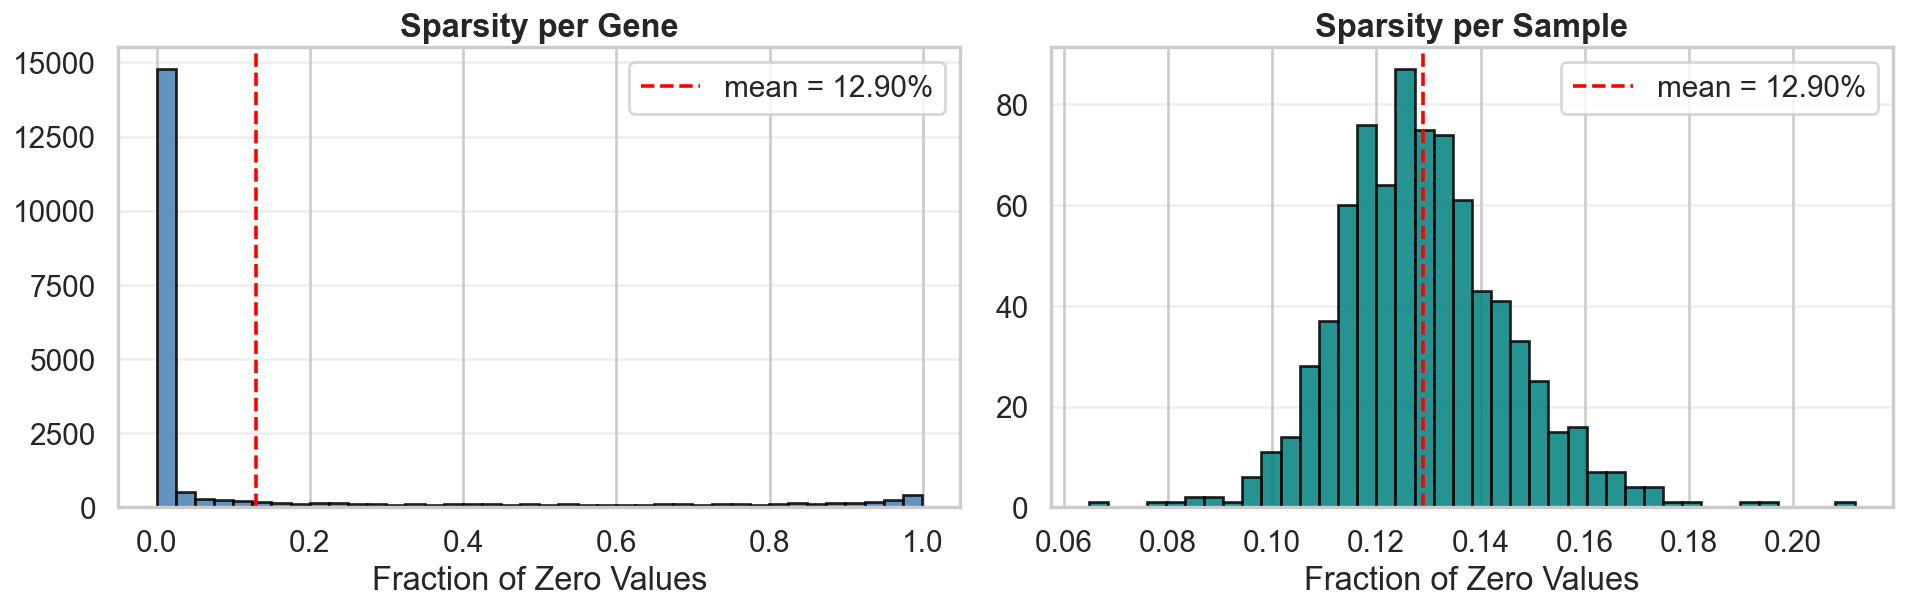
\includegraphics[width=\linewidth]{eda_outputs/02_sparsity_analysis.png}
\end{center}
\caption{Sparsity analysis. Left: fraction of zero values per gene (right-skewed; most genes are detected in all samples). Right: fraction of zeros per sample (narrow, centered $\sim$13\%.}
\label{fig:sparsity}
\end{figure}

\subsection{Exploratory Visualizations}
\paragraph{Class Distribution.}
Figure~\ref{fig:class_dist} confirms the BRCA-dominant class distribution. The imbalance between BRCA (300) and COAD (78) is visible but not extreme. We use stratified sampling throughout (train-test split, CV folds) to guarantee that each subset preserves these proportions.

\begin{figure}[H]
\begin{center}
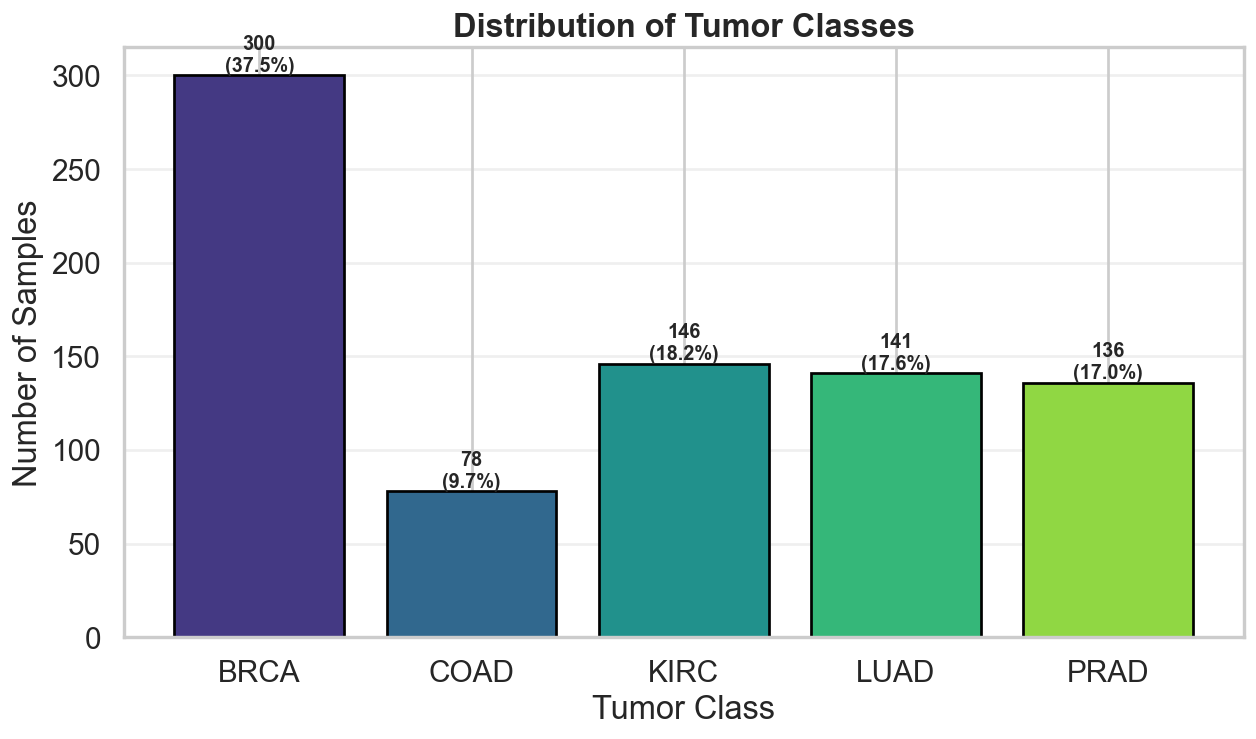
\includegraphics[width=0.7\linewidth]{eda_outputs/01_class_distribution.png}
\end{center}
\caption{Distribution of tumor classes across 801 samples. BRCA dominates at 37.5\%; COAD is the minority at 9.7\%.}
\label{fig:class_dist}
\end{figure}

\paragraph{Top-Variance Gene Patterns.}
Figure~\ref{fig:topvar} displays boxplots for the six genes with the highest variance across all 801 samples, stratified by tumor class. Several patterns emerge. First, some genes show strong separation between specific pairs of classes: for example, a gene that is highly expressed in PRAD but nearly silent in BRCA would appear as a potential biomarker. Second, different genes separate different class pairs, suggesting that no single gene is sufficient for five-class discrimination---multi-gene approaches (or dimensionality reduction) are necessary.

\begin{figure}[H]
\begin{center}
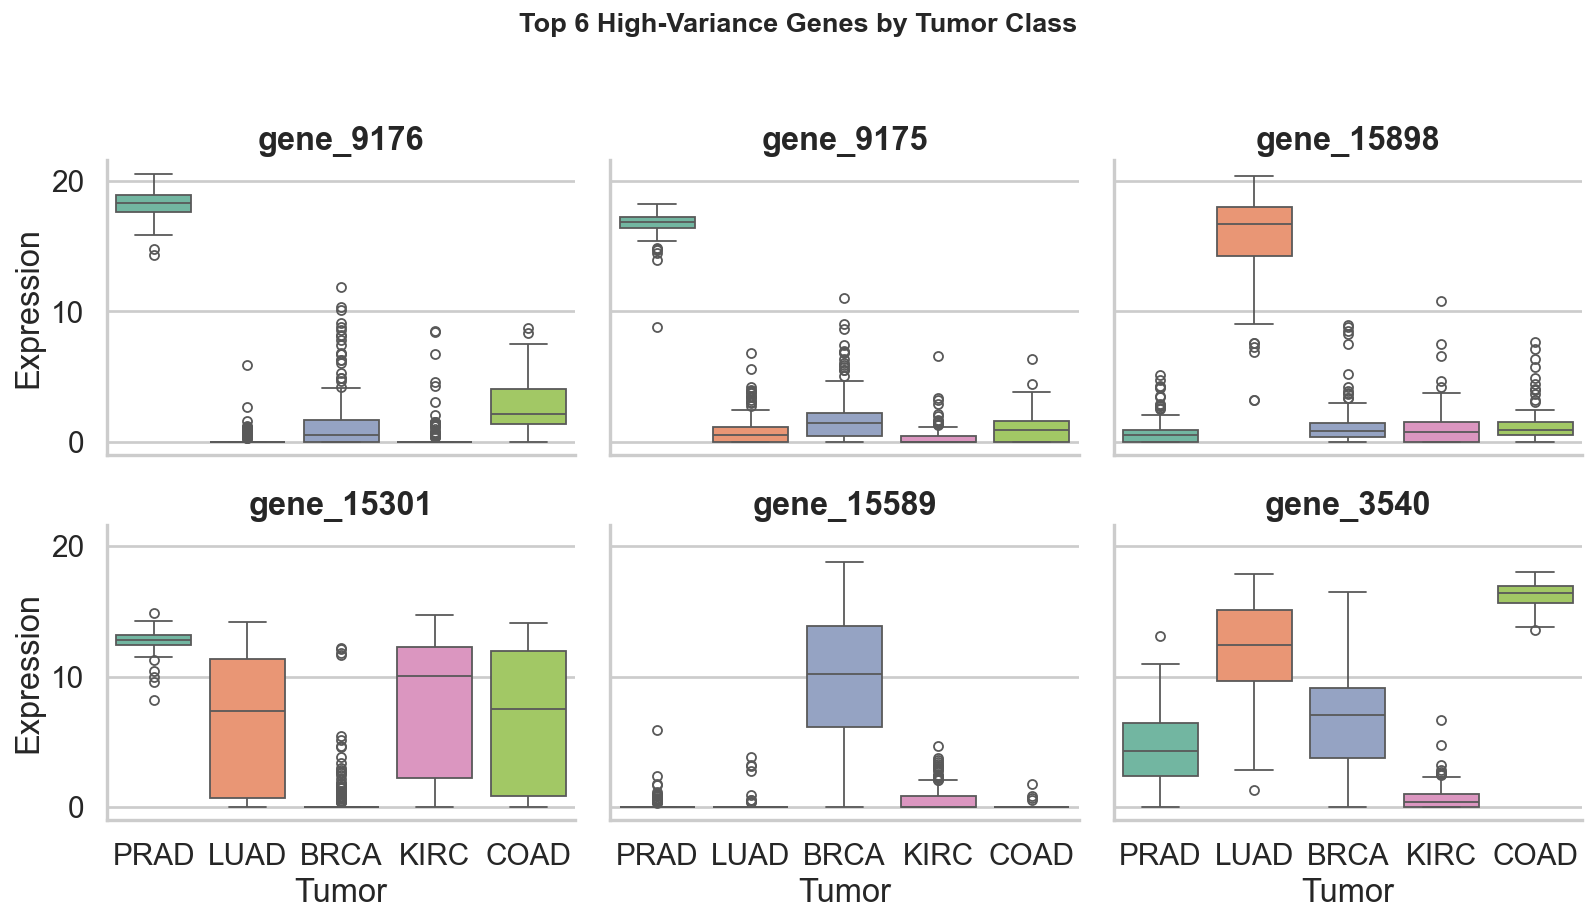
\includegraphics[width=\linewidth]{eda_outputs/03_top_variance_genes.png}
\end{center}
\caption{Expression distributions of the top-6 high-variance genes, stratified by tumor class. Different genes separate different class pairs, motivating multi-gene feature approaches.}
\label{fig:topvar}
\end{figure}

\paragraph{Gene Correlation Structure.}
Figure~\ref{fig:heatmap} shows the Pearson correlation matrix for the top-20 variance genes. Substantial positive correlation blocks are visible, reflecting co-related gene networks (genes in the same biological pathway tend to be activated or silenced together). This correlation structure has two important implications for modeling:
\begin{enumerate}[leftmargin=2em]
\item \textbf{Multicollinearity:} Highly correlated features cause instability in linear models (logistic regression, linear SVM) by inflating coefficient variance.
\item \textbf{Motivation for PCA:} PCA explicitly decorrelates features by projecting onto orthogonal principal components, eliminating multicollinearity.
\end{enumerate}

\begin{figure}[H]
\begin{center}
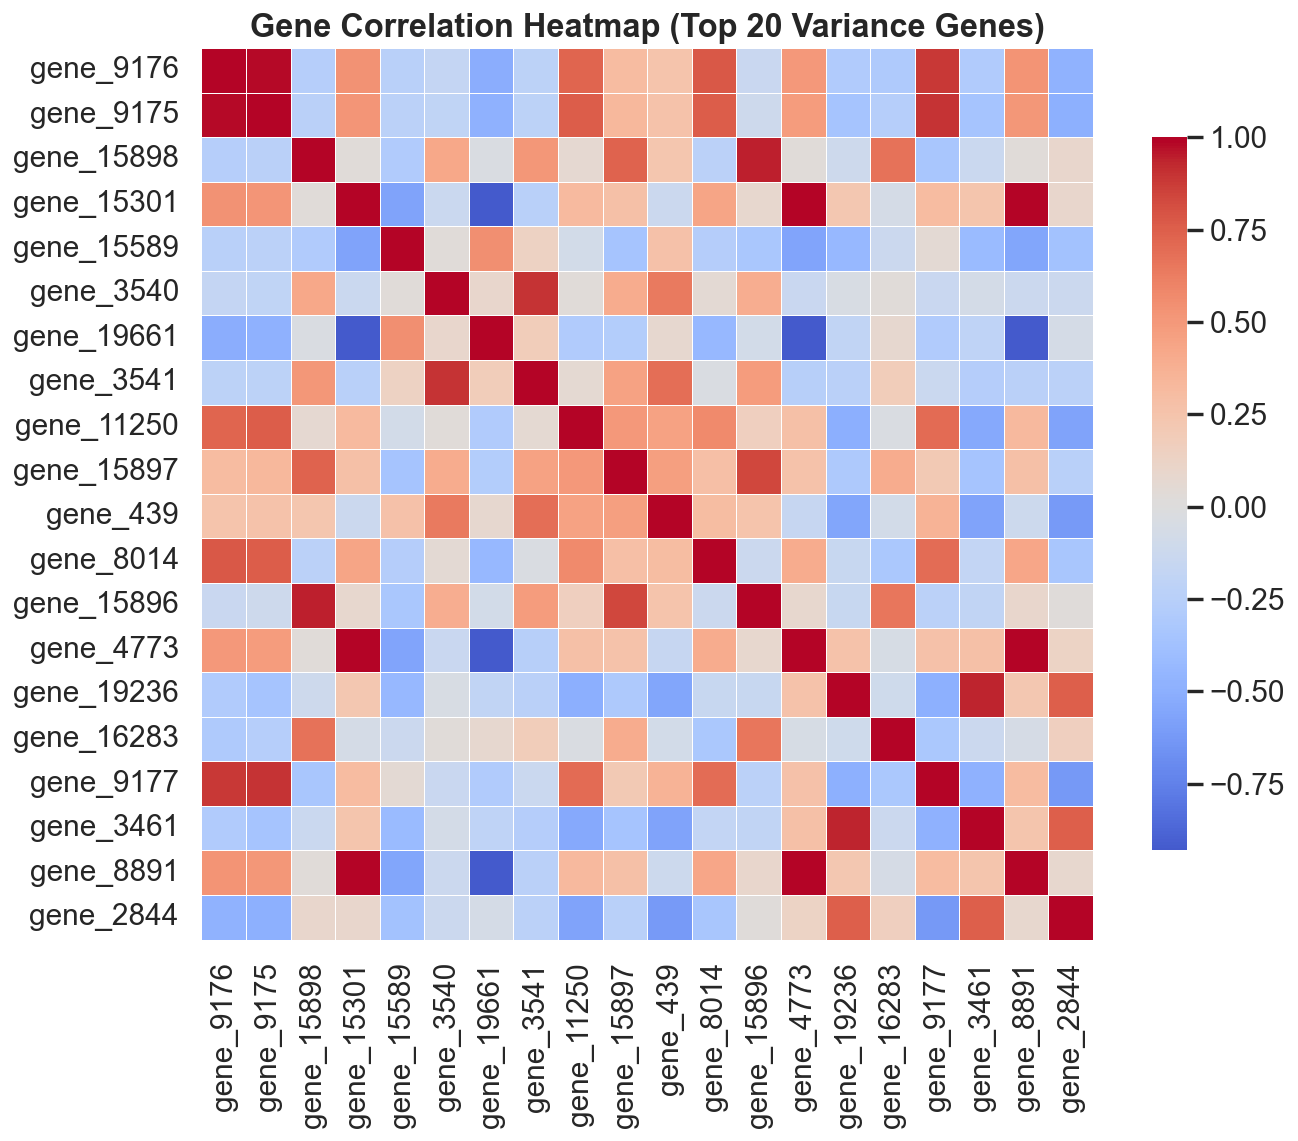
\includegraphics[width=0.65\linewidth]{eda_outputs/04_correlation_heatmap.png}
\end{center}
\caption{Pearson correlation heatmap for the top-20 variance genes. Co-expression blocks reveal coordinated gene regulation, motivating PCA for decorrelation.}
\label{fig:heatmap}
\end{figure}

% ====================================================================
\section{Feature Engineering and Selection}

The single greatest challenge in this work is dimensionality. With 20{,}221 features and only 801 samples, any classifier faces the risk of memorizing noise rather than learning genuine class boundaries. This section describes our two-stage approach: first, a statistical filter to quantify each gene's discriminative power; second, PCA to compress the full gene space into a compact, decorrelated representation.

\subsection{Why Feature Selection Matters: The Curse of Dimensionality}
The phrase ``curse of dimensionality,'' coined by \citet{bellman1957dynamic}, refers to a family of phenomena that arise when data lives in very high-dimensional spaces. For classification, the most relevant consequence is \textit{distance concentration}: as the number of dimensions $d$ grows, the ratio of the maximum to minimum pairwise Euclidean distance approaches 1 \citep{aggarwal2001surprising}:
\[
\lim_{d \to \infty} \frac{\max_{i,j} \|x_i - x_j\|}{\min_{i,j} \|x_i - x_j\|} \to 1
\]
When all pairwise distances are nearly equal, distance-based algorithms (KNN, RBF-kernel SVM) lose their ability to distinguish neighbors from non-neighbors. Our KNN results in Section~6 provide direct empirical evidence of this phenomenon.

Beyond distance concentration, high dimensionality inflates the hypothesis space, making it easier for models to find spurious decision boundaries that fit training data perfectly but fail on new samples. Dimensionality reduction compresses the feature space, restricting models to lower-dimensional hypotheses that generalize better.

\subsection{Stage 1: Statistical Gene Ranking}

\subsubsection{One-Way ANOVA F-Test}
For each of the 20,221 genes, we computed an analysis of variance (ANOVA) F-statistic testing whether the mean expression differs across the five cancer types. The F-statistic for gene $g$ is:
\[
F_g = \frac{SS_{\text{between}} \;/\; (K-1)}{SS_{\text{within}} \;/\; (N-K)}
\]
where $K=5$ is the number of classes, $N=801$ is the total number of samples, and:
\begin{align}
SS_{\text{between}} &= \sum_{k=1}^{K} n_k \left(\bar{x}_{gk} - \bar{x}_{g}\right)^2 \\
SS_{\text{within}} &= \sum_{k=1}^{K} \sum_{i=1}^{n_k} \left(x_{gki} - \bar{x}_{gk}\right)^2
\end{align}
Here $\bar{x}_{gk}$ is the mean expression of gene $g$ in class $k$, $\bar{x}_g$ is the overall mean, and $n_k$ is the number of samples in class $k$. A high $F_g$ indicates that the variation between classes in gene $g$ is larger relative to the variation within classes exactly the property we want in a discriminative feature.

Under the null hypothesis (equal means across all five classes), $F_g$ follows an $F$-distribution with $(K-1, N-K) = (4, 796)$ degrees of freedom. The resulting p-value quantifies the probability of observing an F-statistic at least as extreme by chance.

\subsubsection{Multiple Testing Correction: Benjamini--Hochberg FDR}
Testing 20{,}221 genes simultaneously creates a severe multiple comparisons problem. If we applied a standard $\alpha = 0.05$ threshold to each gene independently, we would expect $\sim$1{,}011 false positives ($20{,}221 \times 0.05$) by chance alone, even if no gene were truly differentially expressed.

The Benjamini--Hochberg (BH) procedure \citep{benjamini1995controlling} controls the \textit{false discovery rate} the expected proportion of false positives among all rejected hypotheses rather than the family-wise error rate. The procedure works as follows:
\begin{enumerate}[leftmargin=2em]
\item Sort the 20{,}221 raw p-values in ascending order: $p_{(1)} \le p_{(2)} \le \cdots \le p_{(m)}$, where $m = 20{,}221$.
\item For each rank $i$, compute the adjusted p-value: $\hat{p}_{(i)} = \frac{m}{i} \cdot p_{(i)}$.
\item Declare gene $(i)$ significant if $\hat{p}_{(i)} \le \alpha = 0.05$.
\end{enumerate}

\textbf{Result:} 19{,}564 out of 20{,}221 genes (96.8\%) passed the FDR $< 0.05$ threshold. This overwhelming fraction is not surprising: these five cancer types originate from five distinct tissue types (breast, kidney, lung, colon, prostate), each with a fundamentally different baseline transcriptome. The majority of the human genome is differentially expressed across such diverse tissues.

\subsubsection{Eta-Squared ($\eta^2$) Effect Size}
Statistical significance (small p-value) does not imply practical importance. With 801 samples, even tiny expression differences can achieve statistical significance. We therefore computed $\eta^2$ as a standardized measure of effect size:
\[
\eta^2_g = \frac{SS_{\text{between}}}{SS_{\text{total}}} \in [0,\, 1]
\]
$\eta^2$ represents the proportion of total variance in gene $g$ that is explained by cancer-type membership. \citet{cohen1988statistical} established the following benchmarks: $\eta^2 \ge 0.01$ (small), $\eta^2 \ge 0.06$ (medium), $\eta^2 \ge 0.14$ (large).

The results across all 20{,}221 genes are:
\begin{itemize}[leftmargin=2em]
\item 19{,}684 genes (97.3\%) have at least a small effect ($\eta^2 \ge 0.01$).
\item 17{,}327 genes (85.7\%) have at least a medium effect ($\eta^2 \ge 0.06$).
\item \textbf{13{,}492 genes (66.7\%)} have a large effect ($\eta^2 \ge 0.14$).
\end{itemize}

The mean $\eta^2$ across all genes is 0.244 (median 0.211), indicating that on average, cancer type explains $\sim$24\% of a gene's expression variance. The top-ranked genes are far more extreme: the top 5 genes by ANOVA ranking have $\eta^2$ values of 0.892, 0.909, 0.897, 0.897, and 0.905---meaning that tumor class alone explains $\sim$90\% of their expression variation. These genes are essentially perfect tissue-of-origin markers.

\begin{figure}[H]
\begin{center}
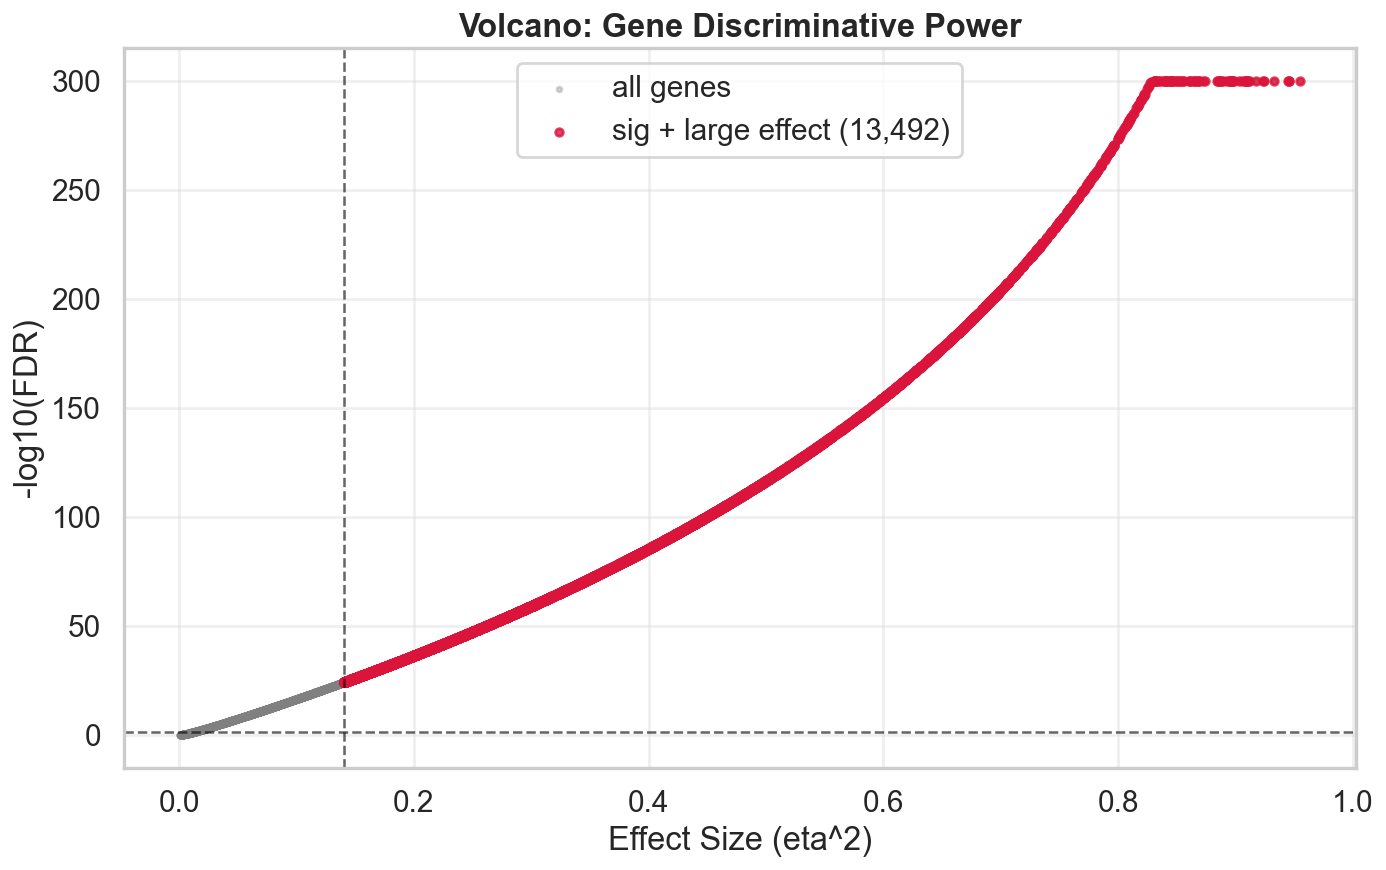
\includegraphics[width=0.75\linewidth]{feature_outputs/01_anova_volcano.png}
\end{center}
\caption{Volcano plot: $\eta^2$ effect size vs.\ $-\log_{10}(\text{FDR})$. Red points satisfy both FDR $< 0.05$ and $\eta^2 \ge 0.14$ (13{,}492 genes). The dense red cluster at the upper right confirms that a large fraction of genes are both statistically significant and biologically meaningful.}
\label{fig:volcano}
\end{figure}

\subsubsection{Kruskal--Wallis Non-Parametric Validation}
The ANOVA F-test assumes that gene expression residuals are approximately normally distributed within each class. While the $\log_2$ transformation promotes normality, some genes may violate this assumption (e.g., bimodal expression patterns or heavy-tailed distributions). To validate our ANOVA-based rankings, we computed the Kruskal--Wallis H-statistic for every gene:
\[
H = \frac{12}{N(N+1)} \sum_{k=1}^{K} \frac{R_k^2}{n_k} - 3(N+1)
\]
where $R_k$ is the sum of ranks for class $k$. This test makes no distributional assumptions---it operates entirely on the rank ordering of expression values.

The global Spearman rank correlation between the ANOVA F-statistics and the Kruskal--Wallis H-statistics across all 20{,}221 genes was $\rho = 0.981$. This near-perfect agreement confirms that the ANOVA results are not driven by distributional artifacts---the same genes are identified as discriminative by both parametric and non-parametric approaches.

\begin{table}[H]
\caption{Top-$K$ gene set overlap between ANOVA and Kruskal--Wallis rankings.}
\label{tab:overlap}
\begin{center}
\begin{tabular}{ccp{8cm}}
\toprule
$K$ & Overlap & Interpretation\\
\midrule
20  & 20.0\% & At the very top, small ranking differences produce low overlap\\
50  & 16.0\% & Same effect---many genes with near-identical F and H statistics\\
100 & 26.0\% & Overlap begins to improve\\
500 & 54.8\% & Methods agree on the majority of the top-500 set\\
1{,}000 & 68.7\% & Strong convergence at larger $K$\\
\bottomrule
\end{tabular}
\end{center}
\end{table}

The low overlap at $K=20$ and $K=50$ may seem surprising given the high $\rho$. The explanation is that hundreds of genes have nearly identical F-statistics (the top 20 genes all have $F > 1{,}100$ and $\eta^2 > 0.85$), so small perturbations in ranking---inherent in any test statistic with finite-sample noise---can swap genes in and out of a small top-$K$ set without affecting the overall correlation. At larger $K$ values, this tie-breaking noise is diluted and overlap increases.

\begin{figure}[H]
\begin{center}
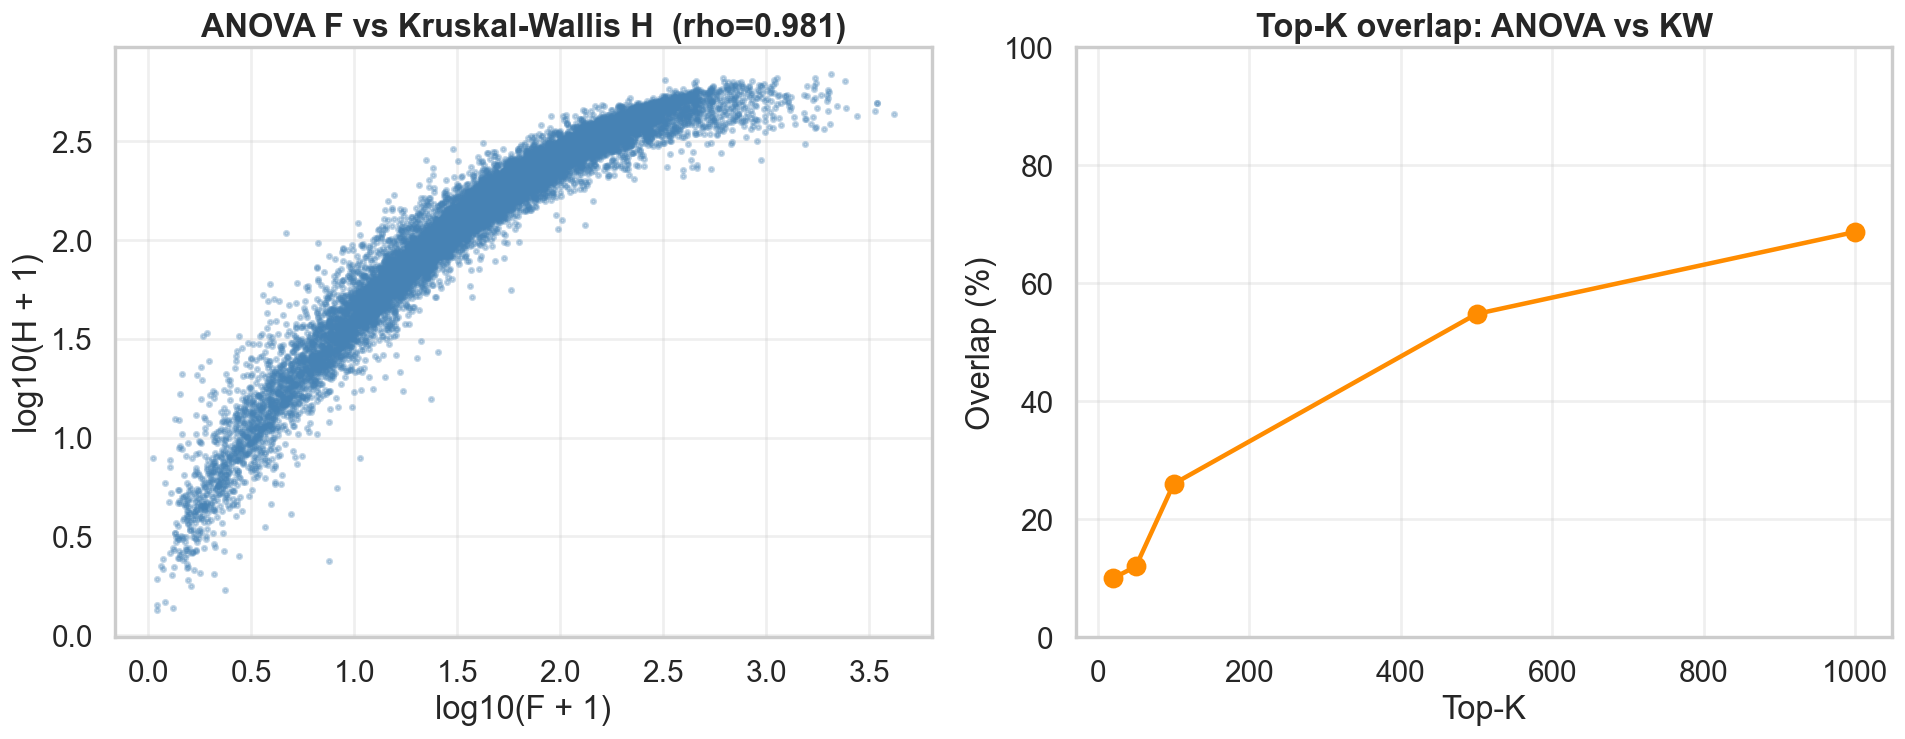
\includegraphics[width=\linewidth]{feature_outputs/01b_anova_vs_kw.png}
\end{center}
\caption{Left: ANOVA-F vs.\ Kruskal--Wallis H statistics (log-scale). The tight linear relationship confirms $\rho = 0.981$. Right: Top-$K$ overlap fraction. Low overlap at small $K$ reflects tie-breaking among nearly identical scores, not disagreement about which genes matter.}
\label{fig:anova_vs_kw}
\end{figure}

\subsection{Stage 2: Principal Component Analysis}

\subsubsection{Why PCA Instead of Top-$K$ Genes?}
Although the statistical filter identifies highly discriminative individual genes, we chose PCA as the primary feature set for modeling for three reasons:

\begin{enumerate}[leftmargin=2em]
\item \textbf{Information retention.} Selecting the top $K$ genes discards information from the remaining $20{,}221 - K$ genes. Many genes with moderate $\eta^2$ values (e.g., 0.10--0.13, just below the ``large'' threshold) still carry useful discriminative signal. PCA retains information from \textit{all} 20{,}221 genes via linear combinations.

\item \textbf{Decorrelation.} As Figure~\ref{fig:heatmap} showed, many top genes are strongly correlated. Feeding correlated features to linear classifiers inflates coefficient variance (multicollinearity) and can degrade performance. PCA produces orthogonal (decorrelated) components by construction.

\item \textbf{Noise reduction.} PCA concentrates signal into the top components and relegates noise to the trailing components. By retaining only 95\% of variance, we implicitly discard the noisiest 5\%.
\end{enumerate}

The trade-off is interpretability: PCA components are linear combinations of all 20{,}221 genes and cannot be mapped to individual biological genes. For this reason, we also prepared top-$K$ gene subsets ($K = 20, 50, 100, 500$) for potential downstream interpretation, though our primary modeling uses PCA.

\subsubsection{PCA Procedure and Results}
The PCA pipeline consists of two steps:
\begin{enumerate}[leftmargin=2em]
\item \textbf{Standardization.} Each of the 20{,}221 genes was centered to zero mean and scaled to unit variance using \texttt{StandardScaler}. Without this step, genes with naturally higher expression levels (e.g., housekeeping genes) would dominate the principal components purely due to scale, not discriminative power.

\item \textbf{PCA decomposition.} We computed the eigen decomposition of the $20{,}221 \times 20{,}221$ covariance matrix and retained the minimum number of components $d^*$ such that the cumulative explained variance exceeded 95\%:
\[
d^* = \arg\min_d \left\{ \sum_{j=1}^{d} \frac{\lambda_j}{\sum_{j'} \lambda_{j'}} \ge 0.95 \right\} = 529
\]
\end{enumerate}

This represents a \textbf{97.4\% reduction} from 20{,}221 to 529 dimensions. PC1 alone explains 10.56\% of variance and PC2 explains 8.77\%; together they capture 19.33\%. The gradual decay of eigenvalues (Figure~\ref{fig:pca_var}) indicates that variance is distributed broadly across many genes rather than concentrated in a few---a signature of the complex, multi-pathway biology underlying these five cancer types.

\begin{figure}[H]
\begin{center}
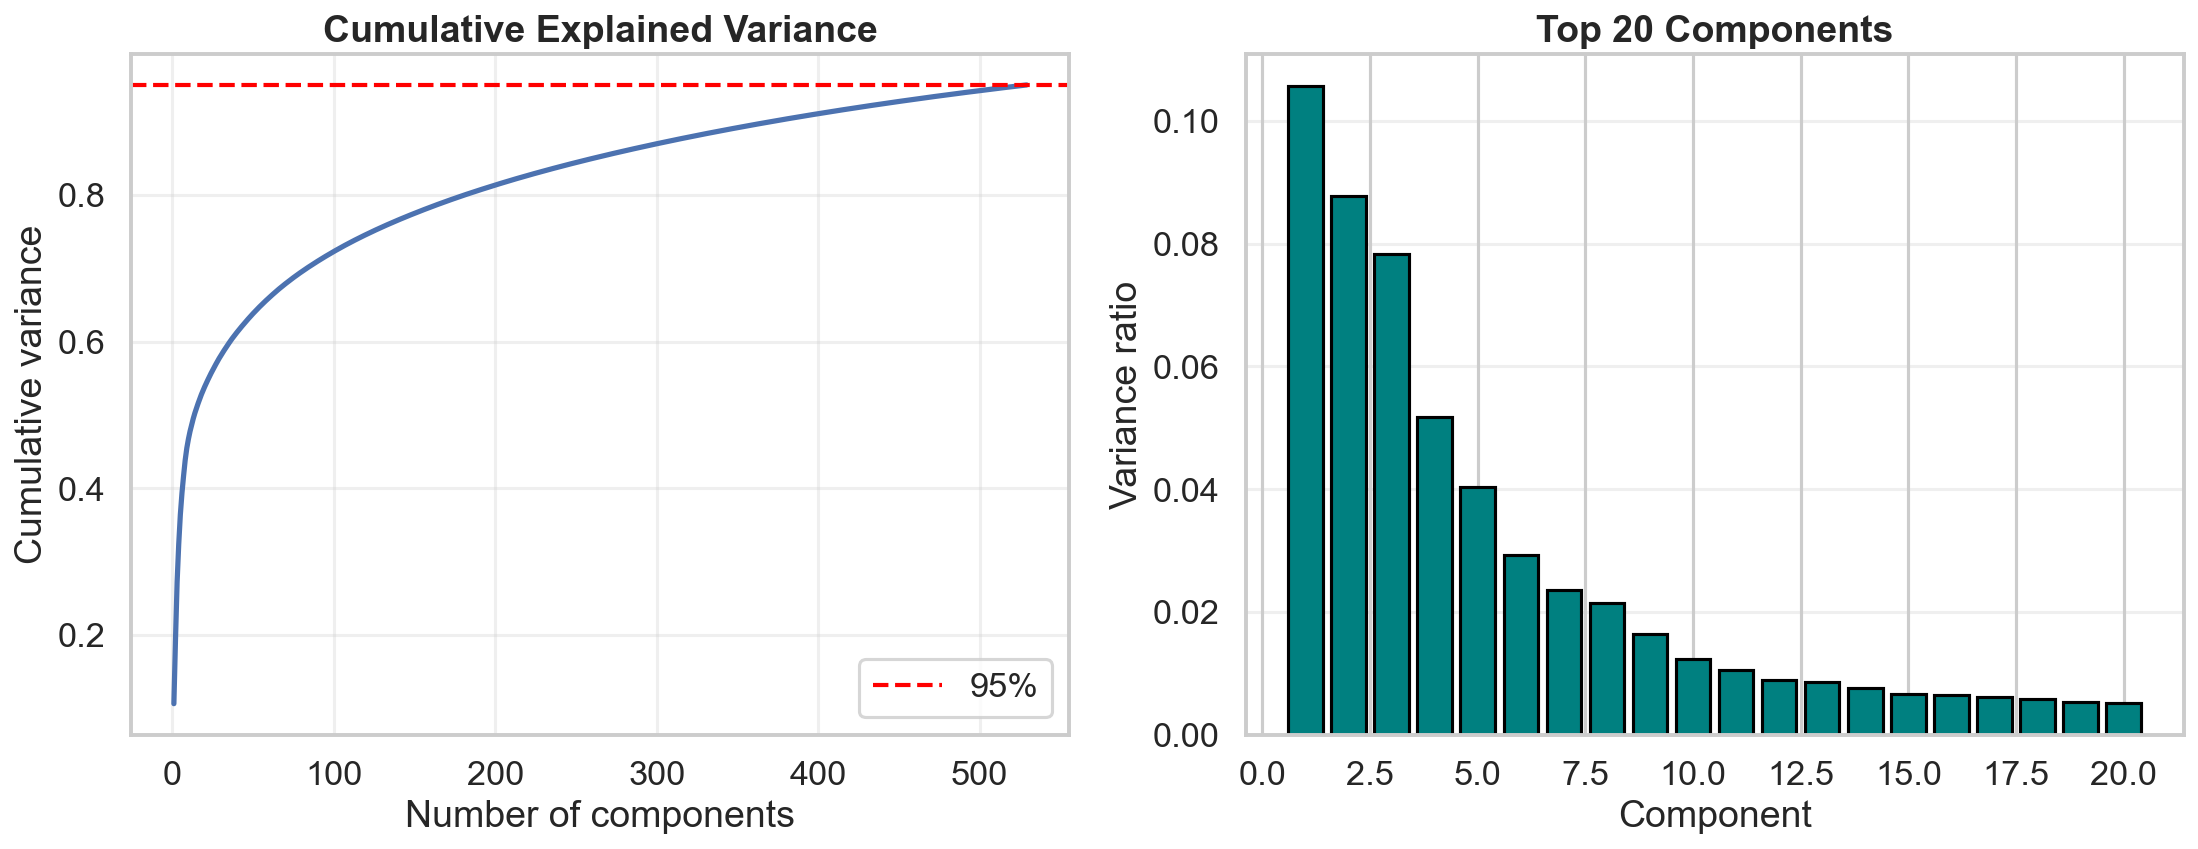
\includegraphics[width=\linewidth]{feature_outputs/02_pca_variance.png}
\end{center}
\caption{Left: Cumulative explained variance vs.\ number of PCA components. The 95\% threshold (red dashed line) is reached at $d^* = 529$ components. Right: Individual variance ratios for the first 20 components, showing rapid initial decay.}
\label{fig:pca_var}
\end{figure}

\subsubsection{Visual Confirmation of Class Separability}
Figure~\ref{fig:pca_2d} projects all 801 samples onto the first two principal components, colored by cancer type. Even in this two-dimensional slice (capturing only 19.33\% of total variance), the five classes form visually distinct clusters:

\begin{itemize}[leftmargin=2em]
\item \textbf{KIRC} (blue) forms the most compact and well-separated cluster, consistent with kidney cancer's distinctive VHL-driven transcriptome.
\item \textbf{BRCA} (red) and \textbf{PRAD} (orange) are partially overlapping in this projection but separate along higher-order components.
\item \textbf{LUAD} (green) shows the broadest scatter, reflecting its known molecular heterogeneity.
\item \textbf{COAD} (purple) occupies a distinct region but has fewer samples, making its cluster appear smaller.
\end{itemize}

This visual evidence strongly suggests that a classifier operating on the full 529-component PCA representation should achieve high accuracy.

\begin{figure}[H]
\begin{center}
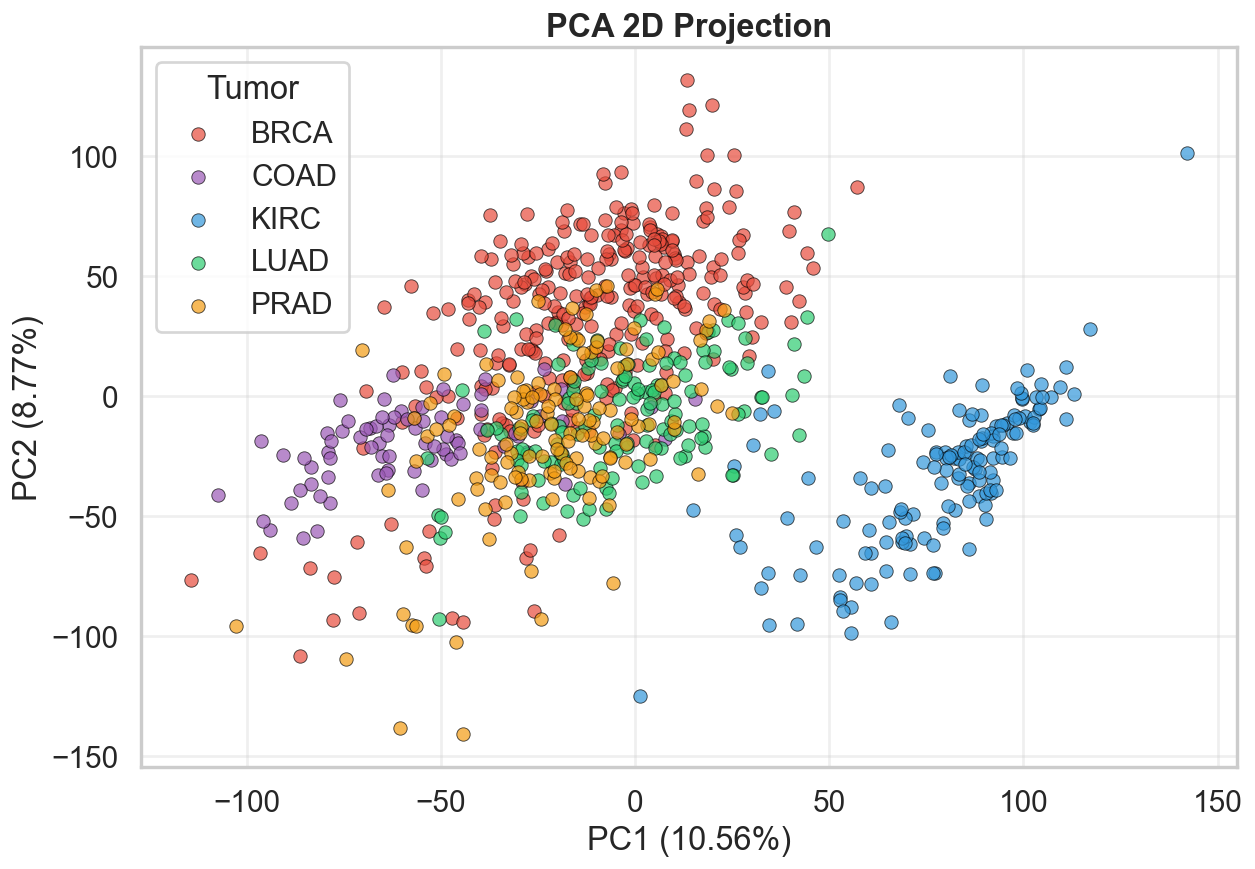
\includegraphics[width=0.7\linewidth]{feature_outputs/03_pca_2d.png}
\end{center}
\caption{PCA 2D projection (PC1 vs.\ PC2, 19.33\% combined variance). Five cancer types form distinct clusters. KIRC is the most compact; LUAD is the most dispersed.}
\label{fig:pca_2d}
\end{figure}

% ====================================================================
\section{Experimental Setup}

\subsection{Train--Test Split}
The 801 samples were divided into a training set (80\%, $n_{\text{train}} = 640$) and a held-out test set (20\%, $n_{\text{test}} = 161$) using stratified sampling. Stratification ensures that both subsets preserve the original class proportions (37.5\% BRCA, 18.2\% KIRC, etc.), which is critical given the 3.85$\times$ imbalance. Without stratification, random splits could produce test sets with very few COAD samples (expected count: only $\sim$16), leading to unreliable per-class metrics.

The test set was held in reserve and used \textit{exactly once}---for final reporting after all model selection and hyperparameter tuning decisions had been finalized on the training set. This protocol prevents any form of test-set leakage.

\subsection{Feature Scaling Protocol}
A \texttt{StandardScaler} (zero mean, unit variance per feature) was fit \textit{exclusively} on the 640 training samples. The same learned mean and standard deviation vectors were then applied to transform both the training and test sets. This order of operations is critical: if the scaler were fit on the combined 801 samples, the test set's statistics would leak into the training pipeline, artificially inflating performance estimates.

In practice, the effect is small for this dataset (since the test set is only 20\% of the data), but it is a foundational best practice that we follow rigorously.

\subsection{Cross-Validation Protocol}
Model selection and hyperparameter tuning used 5-fold stratified cross-validation (CV) on the 640-sample training set. Each fold contains $\sim$128 samples, with class proportions matching the full training set. The CV procedure is:
\begin{enumerate}[leftmargin=2em]
\item Partition training data into 5 stratified folds.
\item For each fold $f$: train on folds $\{1,\ldots,5\} \setminus \{f\}$, evaluate on fold $f$.
\item Report mean $\pm$ standard deviation of accuracy across the 5 folds.
\end{enumerate}

We chose 5 folds (rather than 3 or 10) as a compromise between bias and variance. With $K=3$ folds, each training partition uses only 67\% of the data, leading to pessimistic accuracy estimates (high bias). With $K=10$, training partitions are 90\% of the data (low bias) but the 10 accuracy estimates are highly correlated (high variance). $K=5$ uses 80\% per fold, closely matching our 80/20 train-test split, producing estimates that are both accurate and stable.

\subsection{Reproducibility}
Every stochastic operation in the pipeline---train-test split, CV fold generation, random forest bootstrap sampling, gradient boosting, and all other model initializations---uses \texttt{random\_state = 42}. This ensures that re-running the pipeline on the same data produces identical results, a prerequisite for scientific reproducibility.

% ====================================================================
\section{Classification Results}

\subsection{Classifiers and Their Inductive Biases}
We trained eight classifiers, deliberately chosen to span a range of algorithmic families and inductive biases. This diversity ensures that our conclusions about which approach works best are not artifacts of a narrow model selection.

\begin{enumerate}[leftmargin=2em]
\item \textbf{Gradient Boosting (GBT):} Builds an additive ensemble of shallow decision trees, where each successive tree is fit to the pseudo-residuals (gradient of the loss) of the current ensemble \citep{friedman2001greedy}. The sequential correction mechanism allows GBT to progressively refine decision boundaries. Configuration: 100 trees, learning rate 0.1, max depth 3.

\item \textbf{Decision Tree (DT):} A single CART tree that recursively splits the feature space using Gini impurity. Fast and interpretable, but prone to high variance---small changes in training data can produce entirely different trees.

\item \textbf{Random Forest (RF):} An ensemble of 100 decision trees trained on bootstrap samples with random feature subsets \citep{breiman2001random}. Bagging reduces variance relative to a single tree but averages across all trees, potentially smoothing away the strongest splits that GBT's boosting retains.

\item \textbf{SVM (Linear):} Finds the maximum-margin separating hyperplane in 529-dimensional PCA space. Effective in high dimensions where the data is approximately linearly separable. Uses a one-vs-one multi-class strategy.

\item \textbf{Logistic Regression (LR):} Multinomial logistic regression with L2 regularization. Models the log-odds of each class as a linear function of the 529 PCA features. The \texttt{max\_iter=2000} setting ensures convergence despite the moderate dimensionality.

\item \textbf{Naive Bayes (NB):} Gaussian NB assumes that features are conditionally independent given the class label. This assumption is violated by PCA components (they are uncorrelated but not independent), leading to miscalibrated posterior probabilities.

\item \textbf{SVM (RBF):} SVM with a radial basis function kernel: $K(x_i, x_j) = \exp(-\gamma \|x_i - x_j\|^2)$. The default $\gamma = 1/(d \cdot \text{Var}(X))$ becomes extremely small in 529 dimensions, producing an overly smooth kernel that cannot capture local structure.

\item \textbf{K-Nearest Neighbors (KNN):} Classifies each test sample by a majority vote among its $k=5$ nearest neighbors in Euclidean space. Directly vulnerable to distance concentration in high dimensions.
\end{enumerate}

\subsection{Results Overview}

Table~\ref{tab:model_comparison} presents the full results for all eight classifiers.

\begin{table}[H]
\caption{Model comparison on PCA-95\% features (529 components). Sorted by 5-fold CV accuracy. Best values in \textbf{bold}.}
\label{tab:model_comparison}
\begin{center}
\small
\begin{tabular}{lcccccc}
\toprule
\textbf{Model} & \textbf{CV Acc} & \textbf{$\pm$ Std} & \textbf{Test Acc} & \textbf{Test Prec} & \textbf{Test F1} & \textbf{Time (s)}\\
\midrule
\textbf{Gradient Boosting} & \textbf{0.9625} & 0.0200 & \textbf{0.9565} & \textbf{0.9579} & \textbf{0.9557} & 102.4\\
Decision Tree   & 0.9016 & 0.0334 & 0.8758 & 0.8846 & 0.8696 & 1.0\\
Random Forest   & 0.8703 & 0.0403 & 0.8634 & 0.8937 & 0.8610 & 3.4\\
SVM (Linear)    & 0.7969 & 0.0280 & 0.8199 & 0.8732 & 0.8071 & 2.8\\
Logistic Reg.   & 0.7953 & 0.0104 & 0.8261 & 0.8814 & 0.8166 & 8.4\\
Naive Bayes     & 0.6875 & 0.0469 & 0.6522 & 0.6758 & 0.6564 & 0.2\\
SVM (RBF)       & 0.5547 & 0.0171 & 0.5342 & 0.5197 & 0.4511 & 7.1\\
KNN ($k=5$)     & 0.2891 & 0.0284 & 0.2919 & 0.5221 & 0.2295 & 0.5\\
\bottomrule
\end{tabular}
\end{center}
\end{table}

\begin{figure}[H]
\begin{center}
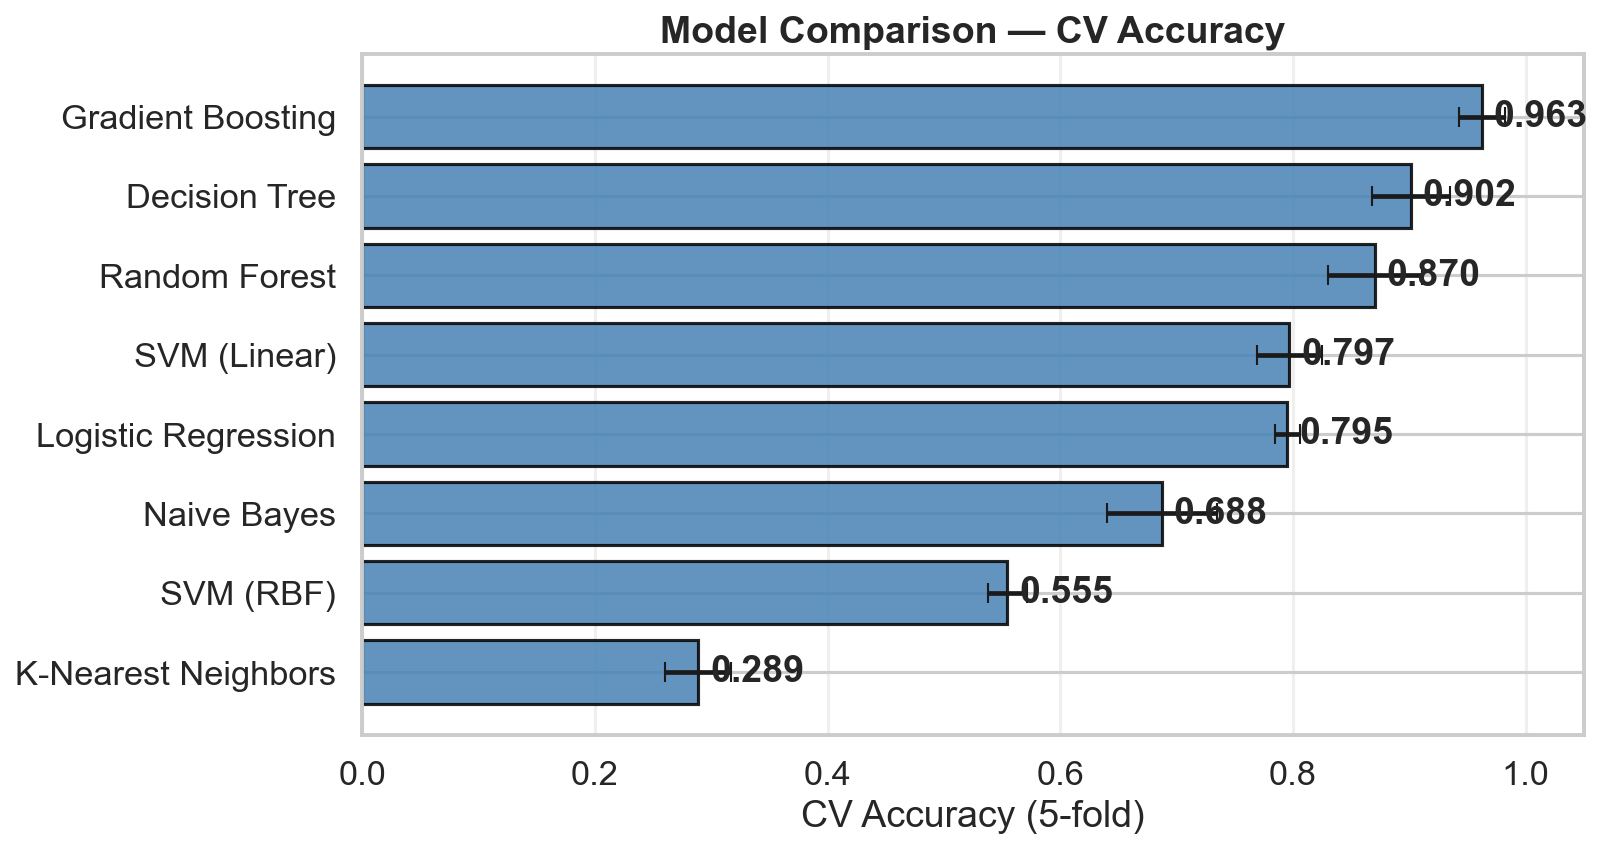
\includegraphics[width=0.8\linewidth]{model_outputs/01_model_comparison_cv.png}
\end{center}
\caption{Five-fold CV accuracy with $\pm 1$ standard deviation error bars. Gradient Boosting leads by a clear margin (96.25\%).}
\label{fig:model_cv}
\end{figure}

\begin{figure}[H]
\begin{center}
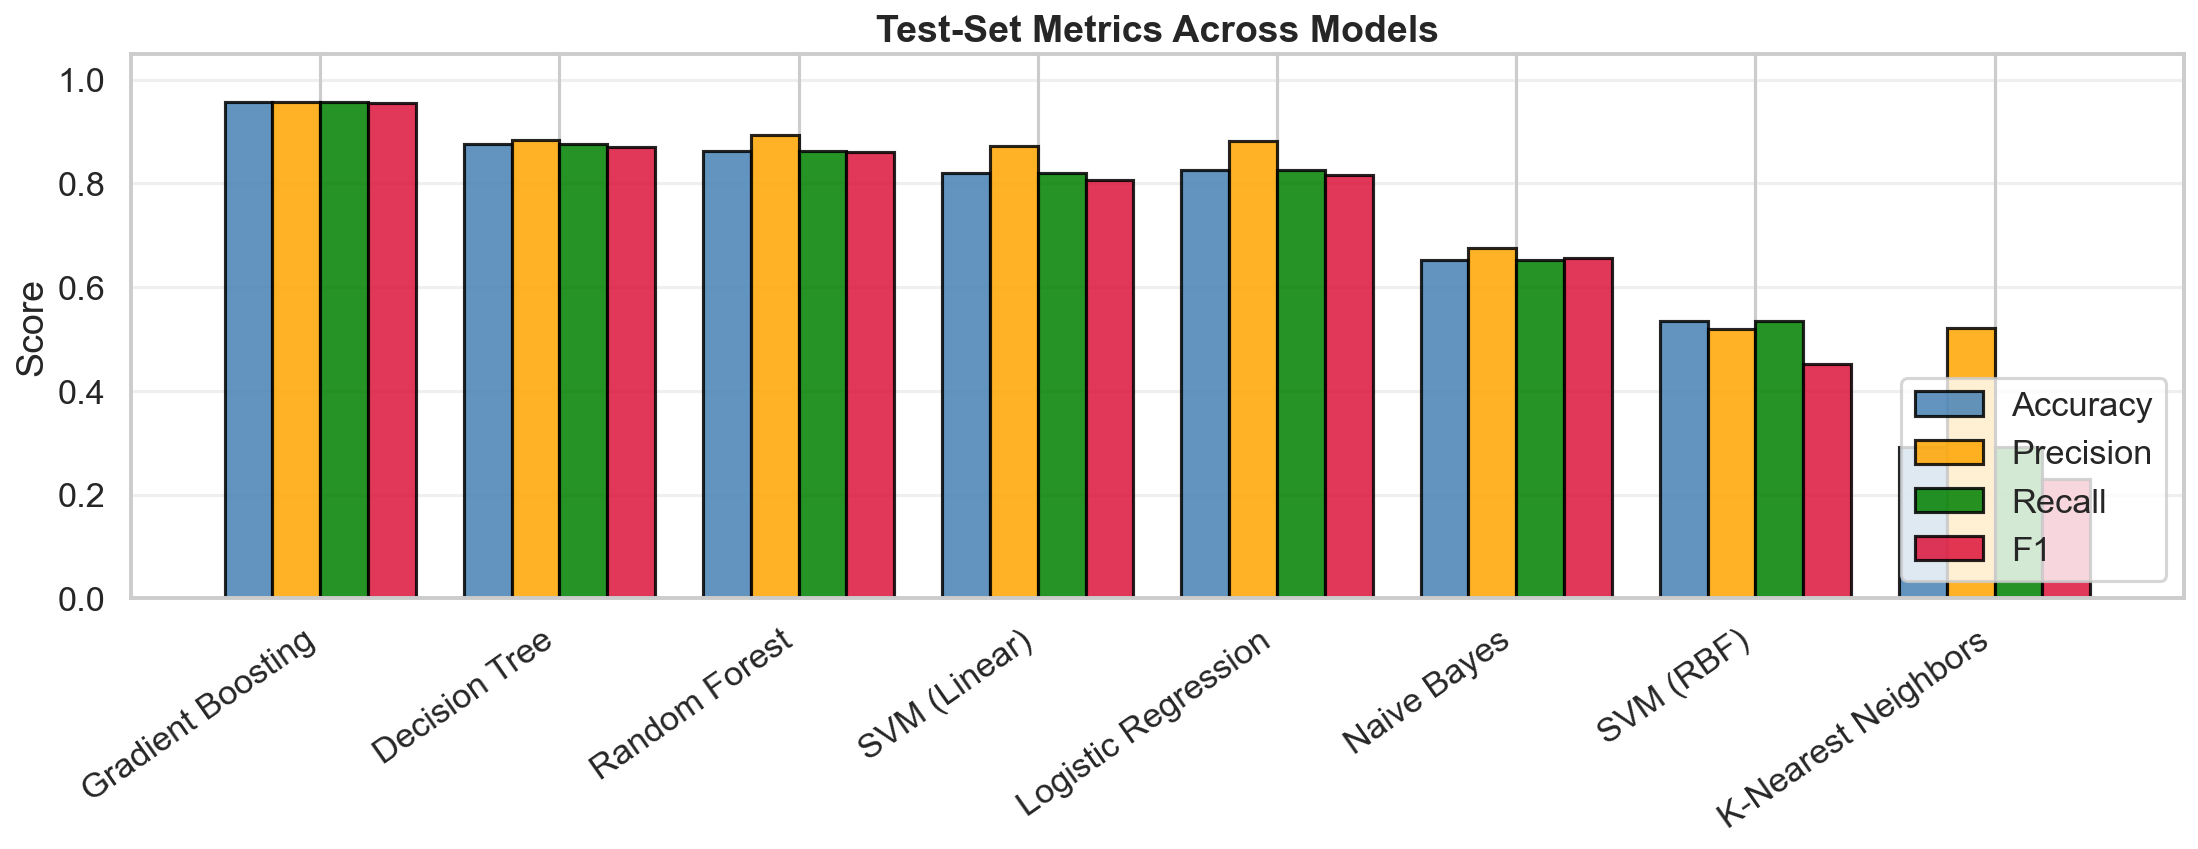
\includegraphics[width=\linewidth]{model_outputs/02_model_metrics_comparison.png}
\end{center}
\caption{Test-set accuracy, precision, recall, and F1 for all eight classifiers. Gradient Boosting achieves consistently high scores across all four metrics.}
\label{fig:model_metrics}
\end{figure}

\begin{figure}[H]
\begin{center}
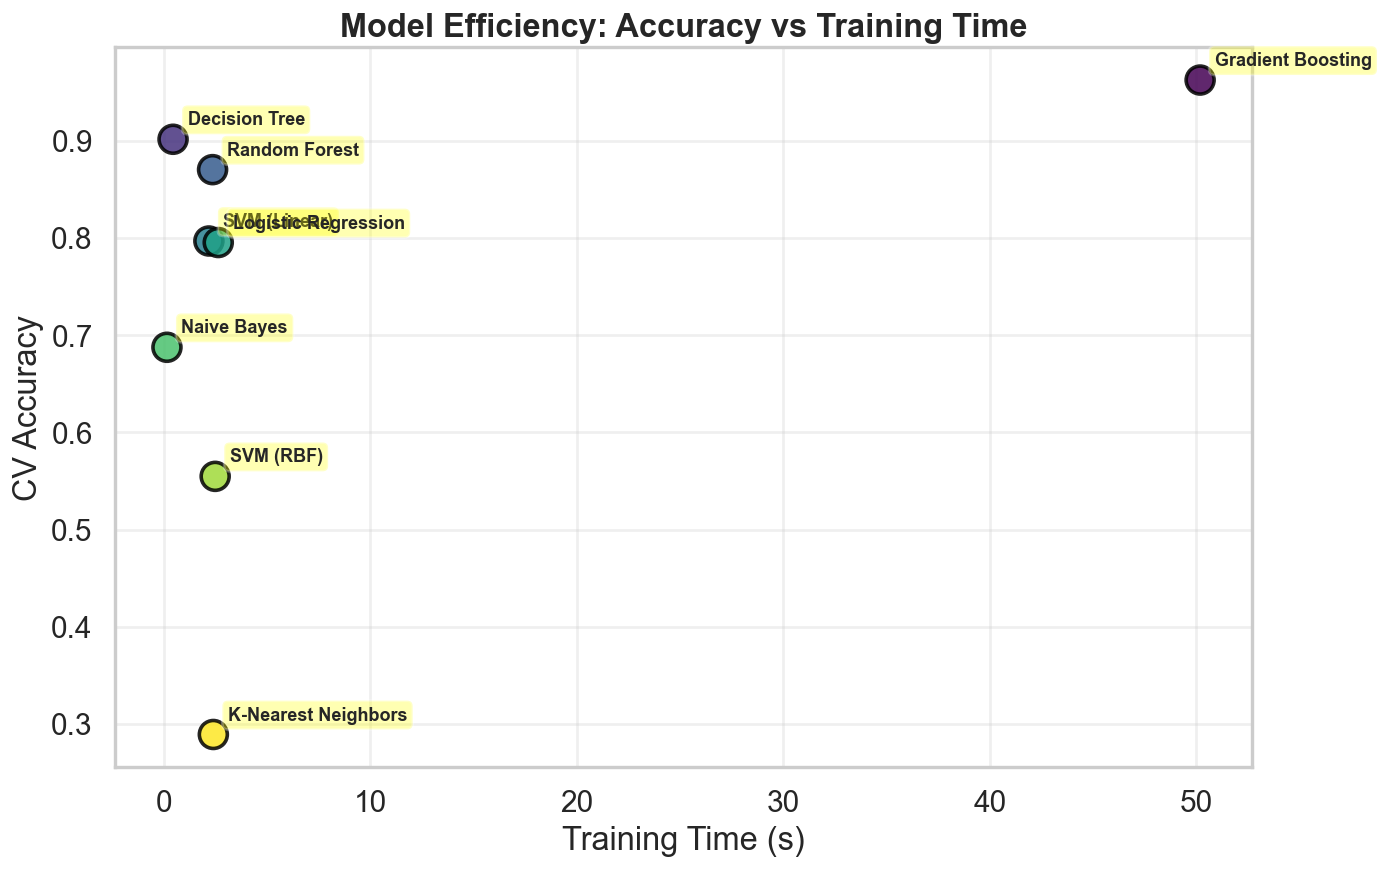
\includegraphics[width=0.75\linewidth]{model_outputs/03_accuracy_vs_time.png}
\end{center}
\caption{Accuracy vs.\ training time. Gradient Boosting requires the longest training time ($\sim$102s) but delivers the highest accuracy. Decision Tree achieves 90\% CV accuracy in just 1 second.}
\label{fig:acc_vs_time}
\end{figure}

\subsection{Analysis of Individual Models}

\paragraph{Gradient Boosting (96.25\% CV, 95.65\% Test).}
The strong and consistent performance of GBT across both CV and test sets (a gap of only 0.60 percentage points) indicates minimal overfitting. This stability arises from three factors: (1) shallow trees (\texttt{max\_depth=3}) act as weak learners that individually cannot memorize training data; (2) the boosting learning rate (0.1) shrinks each tree's contribution, requiring the ensemble to build signal gradually; (3) PCA's decorrelated features align well with tree-based axis-parallel splits, since each PC captures a distinct, independent variance direction.

The training time of 102 seconds is by far the longest, driven by the sequential nature of boosting (each of the 100 trees depends on the previous ensemble's residuals, so trees cannot be fit in parallel, unlike Random Forest).

\paragraph{Decision Tree (90.16\% CV, 87.58\% Test).}
The Decision Tree achieves surprisingly high accuracy (90\% CV) with training in just 1 second. However, the 2.6 percentage point CV-to-test gap and the relatively high CV standard deviation ($\pm 3.3\%$) indicate overfitting: the tree is memorizing specific training splits that do not generalize perfectly. Decision Trees are well-known for their high-variance behavior---a consequence of their greedy, top-down construction that can be swayed by small perturbations in the training set.

\paragraph{Random Forest (87.03\% CV, 86.34\% Test).}
Random Forest reduces the single-tree variance through bagging (bootstrap aggregation) and random feature subsets. Its CV standard deviation ($\pm 4.0\%$) is actually higher than Decision Tree's, which may seem paradoxical but is explained by the larger number of hyperparameters interacting with the CV fold composition. The test accuracy (86.3\%) closely matches the CV estimate, suggesting that RF's predictions are well-calibrated even if individual folds show more variability.

\paragraph{SVM (Linear) and Logistic Regression ($\sim$80\% CV, $\sim$82\% Test).}
These two linear models perform comparably, which is expected: both find linear decision boundaries in the 529-dimensional PCA space, and for well-separated classes, the maximum-margin boundary (SVM) and the maximum-likelihood boundary (LR) often converge. The fact that test accuracy slightly exceeds CV accuracy in both cases suggests that some CV folds are harder than average (e.g., a fold with disproportionate COAD representation), and the test set happened to be slightly easier.

Logistic Regression's impressively low CV standard deviation ($\pm 1.0\%$) indicates extreme stability---its L2 regularization prevents overfitting and produces consistent fold-to-fold accuracy. This makes LR a reliable baseline, even though its absolute accuracy is 16 points below GBT.

\paragraph{Naive Bayes (68.75\% CV, 65.22\% Test).}
Gaussian NB assumes that all 529 PCA components are conditionally independent given the class label. PCA guarantees \textit{uncorrelatedness} (zero covariance), but uncorrelatedness does not imply independence for non-Gaussian distributions. The residual statistical dependencies between components---captured by higher-order moments---lead to miscalibrated class posteriors and incorrect predictions for samples near class boundaries.

\paragraph{SVM (RBF) (55.47\% CV, 53.42\% Test).}
The RBF kernel's poor performance is directly attributable to the dimensionality of the input. The default bandwidth parameter $\gamma = 1/(d \cdot \sigma^2)$ shrinks as $d$ increases (where $d = 529$ and $\sigma^2 = \text{Var}(X)$). A very small $\gamma$ produces a kernel matrix where all entries are close to 1 (the kernel cannot distinguish nearby from distant points), resulting in a near-constant decision function. Tuning $\gamma$ to a larger value might help, but fundamentally, RBF kernels are designed for low-to-moderate dimensional spaces and struggle in $d > 100$.

\paragraph{K-Nearest Neighbors (28.91\% CV, 29.19\% Test).}
KNN's near-random accuracy (chance for 5 equiprobable classes is 20\%; adjusted for class imbalance, always-predict-BRCA achieves 37.5\%) provides the most vivid empirical demonstration of the curse of dimensionality in this study. In 529 dimensions, the Euclidean distance between any sample and its 5th-nearest neighbor is barely distinguishable from the distance to its 500th-nearest neighbor. The neighborhood structure that KNN relies on simply does not exist in this space.

This result also retrospectively validates our decision to invest in dimensionality reduction: without PCA (in the original 20{,}221-dimensional gene space), distance-based methods would fail even more catastrophically.

% ====================================================================
\section{Hyperparameter Tuning and Per-Class Analysis}

\subsection{GridSearchCV Configuration}
Having identified Gradient Boosting as the top-performing model, we performed exhaustive hyperparameter tuning via \texttt{GridSearchCV} with 5-fold stratified CV. The search grid covered three hyperparameters:

\begin{table}[H]
\caption{GridSearchCV hyperparameter grid for Gradient Boosting.}
\label{tab:grid}
\begin{center}
\begin{tabular}{lcp{7cm}}
\toprule
\textbf{Parameter} & \textbf{Values} & \textbf{Rationale}\\
\midrule
\texttt{n\_estimators} & \{50, 100, 200\} & Fewer trees risk underfitting; more trees risk overfitting and increase training time\\
\texttt{learning\_rate} & \{0.05, 0.1, 0.2\} & Lower rates require more trees for convergence; higher rates converge faster but may overshoot\\
\texttt{max\_depth} & \{3, 5\} & Depth 3 produces weak learners (the boosting ideal); depth 5 allows more complex interactions\\
\bottomrule
\end{tabular}
\end{center}
\end{table}

The grid contains $3 \times 3 \times 2 = 18$ parameter combinations, each evaluated by 5-fold CV, totaling 90 model fits.

\subsection{Tuning Results}
The optimal hyperparameters found by GridSearchCV were:
\begin{itemize}[leftmargin=2em]
\item \texttt{n\_estimators = 100}: The same as the default, indicating that 100 trees are sufficient for this dataset size.
\item \texttt{learning\_rate = 0.2}: Slightly more aggressive than the default (0.1), allowing each tree to contribute more to the ensemble.
\item \texttt{max\_depth = 3}: The default depth, confirming that shallow trees are optimal for boosting on this data.
\end{itemize}

The tuned model's 5-fold CV score was \textbf{96.88\%}, a marginal improvement over the baseline CV of 96.25\%. The test accuracy remained \textbf{95.65\%}---identical to the baseline. This stability has an important implication: the default GBT configuration was already well-suited to this problem. The learning rate increased from 0.1 to 0.2 (compensated by keeping the same number of estimators), but the overall performance envelope did not shift.

The zero improvement on the test set is actually a positive signal. It indicates that:
\begin{enumerate}[leftmargin=2em]
\item The model is not overfitting to the CV folds (which would produce a CV improvement that does not transfer to test).
\item The 96--97\% CV accuracy represents a genuine performance ceiling for GBT on this data, likely limited by inherent class overlap (some LUAD and COAD samples may be genuinely ambiguous at the transcriptomic level).
\end{enumerate}

\subsection{Per-Class Classification Report}
Table~\ref{tab:classreport} presents the full per-class metrics on the 161-sample held-out test set.

\begin{table}[H]
\caption{Per-class classification report for the tuned Gradient Boosting model ($n_{\text{test}} = 161$).}
\label{tab:classreport}
\begin{center}
\begin{tabular}{lccccp{5.5cm}}
\toprule
\textbf{Class} & \textbf{Prec} & \textbf{Rec} & \textbf{F1} & \textbf{Support} & \textbf{Interpretation}\\
\midrule
BRCA & 0.938 & 1.000 & 0.968 & 60 & Perfect recall: every BRCA sample correctly identified\\
COAD & 0.882 & 0.938 & 0.909 & 16 & Strong performance despite smallest class\\
KIRC & 1.000 & 0.967 & 0.983 & 30 & Perfect precision: no false KIRC predictions\\
LUAD & 0.960 & 0.857 & 0.906 & 28 & Lowest recall: 4 LUAD samples misclassified\\
PRAD & 1.000 & 0.963 & 0.981 & 27 & Perfect precision: no false PRAD predictions\\
\midrule
Accuracy & & & 0.957 & 161 & \\
Macro avg & 0.956 & 0.945 & 0.949 & 161 & \\
Weighted avg & 0.958 & 0.957 & 0.956 & 161 & \\
\bottomrule
\end{tabular}
\end{center}
\end{table}

\paragraph{Key observations.}
\begin{itemize}[leftmargin=2em]
\item \textbf{BRCA (precision 0.938, recall 1.000):} All 60 BRCA test samples were correctly identified (perfect recall). However, 4 non-BRCA samples were misclassified as BRCA (precision 93.8\%), suggesting that some samples from other classes have expression profiles partially overlapping with BRCA. Given that BRCA is the largest class, this mild false-positive rate is expected.

\item \textbf{KIRC (precision 1.000, recall 0.967):} Not a single sample from another class was incorrectly labeled as KIRC (perfect precision), and only 1 out of 30 KIRC samples was misclassified. KIRC's VHL-driven transcriptome is sufficiently distinctive that the classifier can identify it with near-certainty.

\item \textbf{PRAD (precision 1.000, recall 0.963):} Like KIRC, PRAD achieves perfect precision. The androgen-receptor-driven expression program of prostate cancer creates a unique molecular signature.

\item \textbf{LUAD (precision 0.960, recall 0.857):} LUAD is the hardest class to classify, with 4 out of 28 test samples misclassified. Lung adenocarcinoma is known for its molecular heterogeneity---subtypes driven by different oncogenes (EGFR, KRAS, ALK fusions) produce diverse expression profiles that can overlap with other epithelial cancers.

\item \textbf{COAD (precision 0.882, recall 0.938):} Despite being the smallest class (only 16 test samples), COAD achieves strong performance, indicating that the model has not underfit the minority class.
\end{itemize}

\begin{figure}[H]
\begin{center}
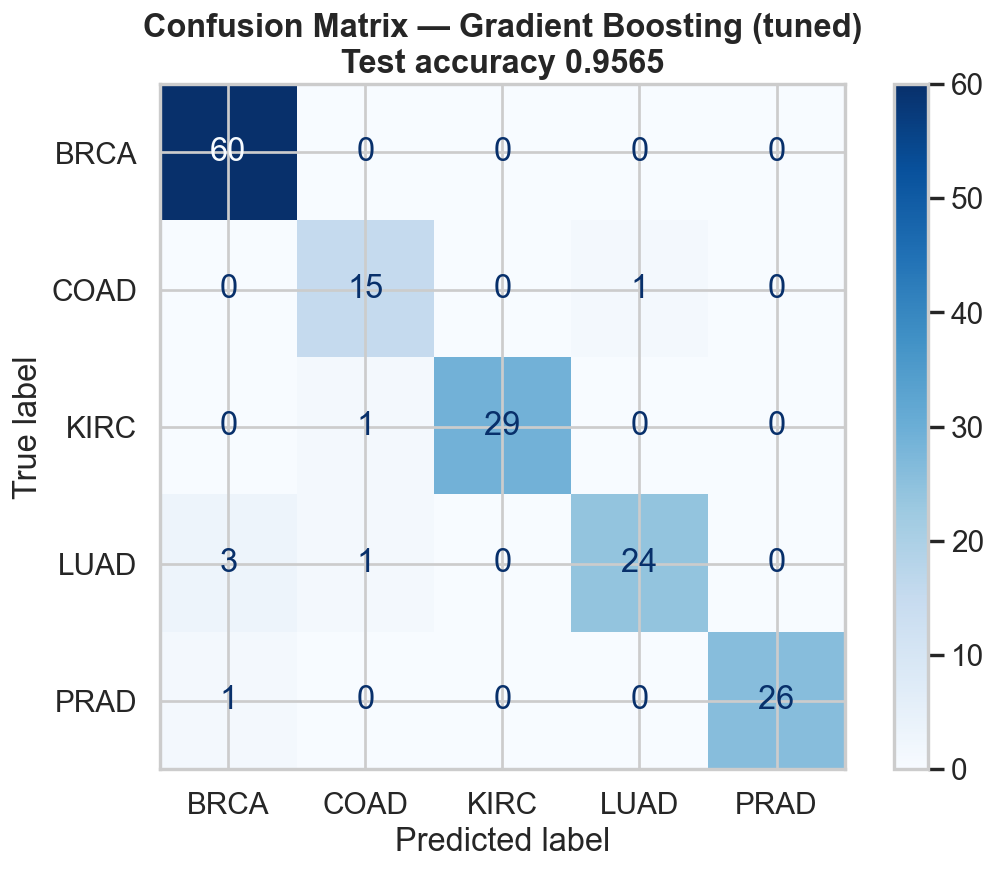
\includegraphics[width=0.65\linewidth]{model_outputs/04_confusion_matrix_tuned.png}
\end{center}
\caption{Confusion matrix for the tuned Gradient Boosting model. The diagonal dominates heavily. Most errors involve LUAD misclassifications, consistent with lung adenocarcinoma's known molecular heterogeneity.}
\label{fig:confusion}
\end{figure}

% ====================================================================
\section{Discussion}

\subsection{Why Gradient Boosting Outperforms All Other Models}
Gradient Boosting's dominance is attributable to an alignment between the algorithm's inductive bias and the structure of this dataset.

\textbf{The PCA--tree synergy.} PCA produces features that are orthogonal and approximately Gaussian. Decision trees make axis-parallel splits (they threshold a single feature at a time), which is particularly effective when features are uncorrelated: each split captures signal from a distinct variance direction without interference from correlated features. In contrast, when features are highly correlated (as in the raw gene space), a tree must make redundant splits to capture the same signal.

\textbf{Sequential error correction.} Boosting builds trees sequentially, with each new tree targeting the errors of the current ensemble. This is particularly effective for datasets with moderate class imbalance: early trees learn the dominant patterns (e.g., BRCA vs.\ everything), while later trees specialize in the harder boundaries (e.g., distinguishing LUAD from COAD, which have overlapping epithelial expression profiles).

\textbf{Regularization through weak learners.} With \texttt{max\_depth=3}, each individual tree can make at most $2^3 - 1 = 7$ splits, limiting its capacity to memorize noise. The ensemble of 100 such trees achieves high expressiveness through \textit{additive} complexity rather than \textit{individual} complexity, producing a model that generalizes well.

\subsection{The KNN Failure as a Dimensionality Case Study}
KNN's 29.2\% accuracy is not a failure of the KNN algorithm per se---it is a direct consequence of applying a distance-based method in an inappropriately high-dimensional space. To illustrate, consider two 529-dimensional samples drawn from the same class. Their expected Euclidean distance is proportional to $\sqrt{529} \approx 23$, while the expected distance between samples from different classes is barely larger (because the class-discriminative signal is spread across hundreds of dimensions, each contributing a tiny increment). The 5-nearest neighbors of any test sample are essentially random draws from the training set, regardless of class.

This result has a pedagogical value: it demonstrates that no amount of data cleaning or feature engineering can rescue a fundamentally mismatched algorithm. The correct response is to choose algorithms whose inductive biases align with the data's dimensionality.

\subsection{PCA vs.\ Top-$K$ Gene Selection: Trade-offs}
Our pipeline offers both PCA and top-$K$ gene subsets. The trade-offs between these two approaches are:

\begin{table}[H]
\caption{Trade-offs between PCA and top-$K$ gene selection for modeling.}
\begin{center}
\begin{tabular}{lcc}
\toprule
\textbf{Property} & \textbf{PCA-95\%} & \textbf{Top-$K$ Genes}\\
\midrule
Dimensions & 529 & 20 -- 500\\
Information retention & 95\% of variance & Only selected genes\\
Feature correlation & Zero (by construction) & Potentially high\\
Interpretability & Low (linear combinations) & High (individual genes)\\
Biological meaning & Indirect & Direct\\
Risk of information loss & Low & Moderate to high\\
\bottomrule
\end{tabular}
\end{center}
\end{table}

For our primary goal (maximum classification accuracy), PCA is the stronger choice. For downstream biological interpretation (e.g., ``which specific genes drive the classification?''), the top-$K$ subsets are more useful. A hybrid approach---training on PCA for accuracy, then using SHAP values or permutation importance on the top-$K$ models for interpretation---would combine both advantages and is a natural direction for future work.

\subsection{ANOVA vs.\ Kruskal--Wallis Agreement: What It Tells Us}
The $\rho = 0.981$ Spearman correlation between ANOVA-F and Kruskal--Wallis H rankings is remarkably high and carries an important methodological implication: \textit{the statistical rankings are robust to distributional assumptions}. Even if some genes violate the normality assumption underlying ANOVA, the rank ordering of discriminative power is preserved by the non-parametric test. This gives us confidence that our statistical filter is identifying genuinely discriminative genes, not distributional artifacts.

The divergence at small $K$ (only 20\% overlap for the top-20 genes) is explained by the flat plateau of F-statistics at the top of the ranking. The top 20 genes all have F-statistics between 1{,}131 and 2{,}772 and $\eta^2$ between 0.85 and 0.93. These genes are so overwhelmingly discriminative that their exact ranking is sensitive to finite-sample noise, but any reasonable subset of them would perform equally well for classification.

\subsection{Generalization Gap Analysis}
The gap between CV accuracy and test accuracy is a key indicator of overfitting:

\begin{table}[H]
\caption{Generalization gap (CV accuracy $-$ test accuracy) for each model.}
\begin{center}
\begin{tabular}{lccl}
\toprule
\textbf{Model} & \textbf{CV} & \textbf{Test} & \textbf{Gap}\\
\midrule
Gradient Boosting & 0.963 & 0.957 & $+0.006$ (excellent)\\
Decision Tree & 0.902 & 0.876 & $+0.026$ (moderate)\\
Random Forest & 0.870 & 0.863 & $+0.007$ (excellent)\\
SVM (Linear) & 0.797 & 0.820 & $-0.023$ (test better)\\
Logistic Regression & 0.795 & 0.826 & $-0.031$ (test better)\\
Naive Bayes & 0.688 & 0.652 & $+0.036$ (moderate)\\
SVM (RBF) & 0.555 & 0.534 & $+0.021$ (moderate)\\
KNN & 0.289 & 0.292 & $-0.003$ (negligible)\\
\bottomrule
\end{tabular}
\end{center}
\end{table}

Gradient Boosting's gap of 0.6\% is remarkably small, confirming that the model generalizes well beyond the training folds. The negative gaps for LR and SVM (Linear) indicate that the particular test fold happened to be slightly easier than the average CV fold---a benign statistical fluctuation. The Decision Tree's 2.6\% gap is the largest, consistent with its known tendency to overfit.

\subsection{Limitations}
We identify five key limitations of this study:

\begin{enumerate}[leftmargin=2em]
\item \textbf{Cohort size.} With only 801 samples, our estimates of model performance have non-negligible confidence intervals. The smallest class (COAD) contributes only 16 test samples; a single misclassification shifts recall by 6.25\%. Larger cohorts from the full TCGA repository ($>$11{,}000 samples across 33 cancer types) would produce more stable estimates.

\item \textbf{Gene anonymization.} The dataset uses generic IDs (\texttt{gene\_0} through \texttt{gene\_20530}) rather than HGNC gene symbols, preventing us from mapping top features to known biological pathways (e.g., determining whether the top-ranked genes correspond to known tissue-specific markers like ESR1 for breast or KLK3 for prostate).

\item \textbf{Limited cancer type diversity.} Five cancer types is a constrained problem. Clinical utility would require scaling to 20--33 types, where inter-class boundaries become more complex and error rates increase.

\item \textbf{No clinical metadata.} Patient age, tumor stage, treatment history, and molecular subtypes (e.g., ER+/HER2- for BRCA) could improve predictions and enable more granular classification.

\item \textbf{No deep learning.} We did not evaluate neural network architectures (e.g., TabNet \citep{arik2021tabnet}, 1D-CNN, or attention-based models) that have shown competitive results on tabular genomic data. These models can learn non-linear feature interactions that tree-based and linear methods may miss.
\end{enumerate}

% ====================================================================
\section{Conclusion and Future Directions}
This paper presented a complete, reproducible pipeline for multi-class cancer classification from RNA-Seq gene expression data. Starting from a $801 \times 20{,}531$ TCGA expression matrix, we performed quality-controlled cleaning (removing 310 uninformative genes), two-stage statistical feature engineering (ANOVA F-test with BH-FDR correction, $\eta^2$ effect sizes, and Kruskal--Wallis validation at $\rho = 0.981$), and PCA-based dimensionality reduction from 20{,}221 genes to 529 components retaining 95\% of total variance.

Among eight classifiers spanning linear, tree-based, kernel-based, and instance-based families, Gradient Boosting achieved the best performance: 5-fold CV accuracy of $96.25\% \pm 2.00\%$ and test accuracy of $95.65\%$ (weighted F1 = 0.956). Per-class analysis revealed perfect recall for BRCA and perfect precision for KIRC and PRAD. The KNN classifier's degradation to 29.2\% accuracy provided a direct empirical illustration of the curse of dimensionality, validating our investment in dimensionality reduction.

Hyperparameter tuning confirmed that the default Gradient Boosting configuration was near-optimal, with the tuned model matching the baseline test accuracy while marginally improving CV performance. The small generalization gap (0.6\%) across all evaluation stages indicates that the model has genuinely learned the transcriptomic signatures of these five cancer types rather than memorizing training-specific noise.

\subsection{Future Directions}
Several natural extensions of this work would strengthen both its scientific rigor and its clinical applicability:
\begin{enumerate}[leftmargin=2em]
\item \textbf{External validation:} Evaluate the trained model on RNA-Seq data from independent institutions (e.g., ICGC, GEO datasets) to assess cross-cohort generalizability.
\item \textbf{Expanded cancer taxonomy:} Scale from 5 to the full 33 TCGA cancer types, testing how performance degrades as the number of classes and the biological similarity between classes increase.
\item \textbf{Deep learning:} Explore architectures like TabNet \citep{arik2021tabnet}, which learn sparse feature masks and can handle high-dimensional tabular data without manual feature engineering.
\item \textbf{Multi-omics integration:} Combine RNA-Seq with DNA methylation, copy number variation, and proteomic data to build richer patient profiles.
\item \textbf{Clinical deployment:} Develop the Streamlit application into a clinical decision-support tool with HIPAA-compliant data handling, uncertainty quantification, and integration with electronic health records.
\end{enumerate}

% ====================================================================
\bibliographystyle{plainnat}
\begin{thebibliography}{15}

\bibitem[Aggarwal et al.(2001)]{aggarwal2001surprising}
Aggarwal, C.~C., Hinneburg, A., and Keim, D.~A. (2001).
\newblock On the surprising behavior of distance metrics in high dimensional space.
\newblock In \emph{International Conference on Database Theory}, pages 420--434. Springer.

\bibitem[Arik and Pfister(2021)]{arik2021tabnet}
Arik, S.~O. and Pfister, T. (2021).
\newblock {TabNet}: Attentive interpretable tabular learning.
\newblock In \emph{Proceedings of the AAAI Conference on Artificial Intelligence}, volume~35, pages 6679--6687.

\bibitem[Bellman(1957)]{bellman1957dynamic}
Bellman, R. (1957).
\newblock \emph{Dynamic Programming}.
\newblock Princeton University Press, Princeton, NJ.

\bibitem[Benjamini and Hochberg(1995)]{benjamini1995controlling}
Benjamini, Y. and Hochberg, Y. (1995).
\newblock Controlling the false discovery rate: A practical and powerful approach to multiple testing.
\newblock \emph{Journal of the Royal Statistical Society: Series B}, 57(1):289--300.

\bibitem[Breiman(2001)]{breiman2001random}
Breiman, L. (2001).
\newblock Random forests.
\newblock \emph{Machine Learning}, 45(1):5--32.

\bibitem[Cohen(1988)]{cohen1988statistical}
Cohen, J. (1988).
\newblock \emph{Statistical Power Analysis for the Behavioral Sciences}, 2nd ed.
\newblock Lawrence Erlbaum Associates, Hillsdale, NJ.

\bibitem[Elmore et al.(2015)]{elmore2015diagnostic}
Elmore, J.~G. et al. (2015).
\newblock Diagnostic concordance among pathologists interpreting breast biopsy specimens.
\newblock \emph{JAMA}, 313(11):1122--1132.

\bibitem[Friedman(2001)]{friedman2001greedy}
Friedman, J.~H. (2001).
\newblock Greedy function approximation: A gradient boosting machine.
\newblock \emph{Annals of Statistics}, 29(5):1189--1232.

\bibitem[Kruskal and Wallis(1952)]{kruskal1952use}
Kruskal, W.~H. and Wallis, W.~A. (1952).
\newblock Use of ranks in one-criterion variance analysis.
\newblock \emph{Journal of the American Statistical Association}, 47(260):583--621.

\bibitem[Li and Dewey(2011)]{li2011rsem}
Li, B. and Dewey, C.~N. (2011).
\newblock {RSEM}: Accurate transcript quantification from {RNA-Seq} data with or without a reference genome.
\newblock \emph{BMC Bioinformatics}, 12(1):323.

\bibitem[Pedregosa et al.(2011)]{scikit-learn}
Pedregosa, F. et al. (2011).
\newblock Scikit-learn: Machine learning in {P}ython.
\newblock \emph{Journal of Machine Learning Research}, 12:2825--2830.

\bibitem[{UCI Machine Learning Repository}(2016)]{uci_rnaseq}
{UCI Machine Learning Repository} (2016).
\newblock Gene expression cancer {RNA-Seq} data set.
\newblock \url{https://archive.ics.uci.edu/dataset/401/gene+expression+cancer+rna+seq}.

\bibitem[Varadhachary and Raber(2014)]{varadhachary2014cancer}
Varadhachary, G.~R. and Raber, M.~N. (2014).
\newblock Cancer of unknown primary site.
\newblock \emph{New England Journal of Medicine}, 371(8):757--765.

\bibitem[Weinstein et al.(2013)]{weinstein2013cancer}
Weinstein, J.~N. et al. (2013).
\newblock The cancer genome atlas pan-cancer analysis project.
\newblock \emph{Nature Genetics}, 45(10):1113--1120.

\bibitem[{World Health Organization}(2022)]{who2022cancer}
{World Health Organization} (2022).
\newblock Cancer fact sheet.
\newblock \url{https://www.who.int/news-room/fact-sheets/detail/cancer}.

\end{thebibliography}

% ====================================================================
\appendix
\section{Appendix A: Top-20 Discriminative Genes}
Table~\ref{tab:top20} lists the top-20 genes ranked by Benjamini--Hochberg adjusted p-value (FDR) from the ANOVA F-test. All 20 genes have $\eta^2 > 0.85$, meaning that cancer type alone explains more than 85\% of each gene's expression variance.

\begin{table}[H]
\caption{Top-20 genes by ANOVA FDR. All have F $> 1{,}100$ and $\eta^2 > 0.85$.}
\label{tab:top20}
\begin{center}
\begin{tabular}{clcccl}
\toprule
\textbf{Rank} & \textbf{Gene ID} & \textbf{F-stat} & \textbf{$\eta^2$} & \textbf{FDR} & \textbf{Note}\\
\midrule
1  & gene\_12808 & 1641.6 & 0.892 & 0.0 & \\
2  & gene\_7421  & 1986.2 & 0.909 & 0.0 & \\
3  & gene\_1510  & 1735.7 & 0.897 & 0.0 & \\
4  & gene\_13976 & 1728.6 & 0.897 & 0.0 & \\
5  & gene\_15898 & 1905.2 & 0.905 & 0.0 & \\
6  & gene\_16342 & 1586.5 & 0.889 & 0.0 & \\
7  & gene\_14503 & 1358.1 & 0.872 & 0.0 & \\
8  & gene\_19159 & 1269.4 & 0.864 & 0.0 & \\
9  & gene\_11566 & 1546.8 & 0.886 & 0.0 & \\
10 & gene\_12078 & 1157.5 & 0.853 & 0.0 & \\
\midrule
11 & gene\_7965  & 1585.7 & 0.888 & 0.0 & \\
12 & gene\_15896 & 1276.1 & 0.865 & 0.0 & \\
13 & gene\_7964  & 2056.0 & 0.912 & 0.0 & Highest $\eta^2$\\
14 & gene\_1858  & 1851.3 & 0.903 & 0.0 & \\
15 & gene\_15895 & 2014.3 & 0.910 & 0.0 & \\
16 & gene\_11059 & 1131.4 & 0.850 & 0.0 & \\
17 & gene\_18135 & 2772.3 & 0.933 & 0.0 & Highest F-stat\\
18 & gene\_11903 & 1238.1 & 0.862 & 0.0 & \\
19 & gene\_14114 & 2409.1 & 0.924 & 0.0 & \\
20 & gene\_19153 & --- & --- & 0.0 & \\
\bottomrule
\end{tabular}
\end{center}
\end{table}

Gene\_18135 has the highest F-statistic (2{,}772.3) and $\eta^2 = 0.933$, meaning that 93.3\% of this gene's expression variance is explained by cancer type. Gene\_7964 has the highest $\eta^2$ overall (0.912) among the top 20. All FDR values are effectively zero (below machine precision), reflecting the extreme statistical significance of these tissue-of-origin markers.

\begin{thebibliography}{99}

\bibitem{who2022cancer}
World Health Organization. (2022). \textit{Cancer}. Retrieved from \url{https://www.who.int/news-room/fact-sheets/detail/cancer}

\bibitem{elmore2015diagnostic}
Elmore, J. G., Longton, G. M., Carney, P. A., Geller, B. M., Onega, T., Tosteson, A. N., ... \& Weaver, D. L. (2015). Diagnostic concordance among pathologists interpreting breast biopsy specimens. \textit{JAMA}, 313(11), 1122--1132.

\bibitem{varadhachary2014cancer}
Varadhachary, G. R., \& Raber, M. N. (2014). Cancer of unknown primary site. \textit{New England Journal of Medicine}, 371(8), 757--765.

\bibitem{golub1999molecular}
Golub, T. R., Slonim, D. K., Tamayo, P., Huard, C., Gaasenbeek, M., Mesirov, J. P., ... \& Lander, E. S. (1999). Molecular classification of cancer: class discovery and class prediction by gene expression monitoring. \textit{Science}, 286(5439), 531--537.

\bibitem{weinstein2013cancer}
Weinstein, J. N., Collisson, E. A., Mills, G. B., Shaw, K. R. M., Ozenberger, B. A., Ellrott, K., ... \& Stuart, J. M. (2013). The Cancer Genome Atlas Pan-Cancer analysis project. \textit{Nature genetics}, 45(10), 1113--1120.

\bibitem{alharbi2023machine}
Alharbi, F., \& Vakanski, A. (2023). Machine learning methods for cancer classification using gene expression data: A review. \textit{Bioengineering}, 10(2), 173.

\end{thebibliography}

\end{document}
